% Notes on the writing of the Master Thesis
% Book: How to Write a Lot, Paul Silvia, 2nd Edition
% Book: Getting Things Done, David Allen
%
%
% Mögliche Abgrenzung von anderen: Den hybriden Ansatz von SBST mit DSE verwenden, 
% so wie im Paper von Baars et al.
%
% Mögliche weitere Evaluation: Vergleiche die Coverage von generierten Tests zu der 
% Coverage von manuell geschriebenen Tests von Entwicklern in evaluierten Programmen.
% 

\documentclass{article}
% Please do not change this options...
\usepackage[a4paper, total={6in, 10in}]{geometry}
\usepackage{graphicx}
\graphicspath{ {./img/} }
\usepackage{todonotes}
\usepackage{acronym}
\usepackage{float}
\usepackage{algorithm}
\usepackage{amsmath}
\usepackage{amssymb}
\usepackage[shortlabels]{enumitem}

\usepackage{algpseudocode}
\algblock{Input}{EndInput}
\algnotext{EndInput}
\algblock{Output}{EndOutput}
\algnotext{EndOutput}
\newcommand{\Desc}[2]{\State \makebox[2em][l]{#1}#2}
\usepackage[T1]{fontenc}
\makeatletter
\newcommand\BeraMonottfamily{%
  \def\fvm@Scale{0.85}% scales the font down
  \fontfamily{fvm}\selectfont% selects the Bera Mono font
}
\makeatother


\usepackage{listings,multicol}
\lstset{
  numbers=left,
  xleftmargin=2.5em,
  framexleftmargin=2.5em,
  frame=tb,
  stepnumber=1,    
  firstnumber=1,
  numberfirstline=true,
  basicstyle=\BeraMonottfamily,
  identifierstyle=,
  stringstyle=\ttfamily,
  %keywordstyle=\color{OliveGreen},
  keywordstyle=,
  showstringspaces=false
}

% This package must be declared last
\usepackage{cleveref}

\begin{document}

\title{Master Thesis}
\author{Vsevolod Tymofyeyev}
\date{\today}
\maketitle

\tableofcontents
\newpage
\section{Introduction}
In the programming language world, there are two major sides. There are low-level languages that offer better performance at the expense of security and high-level languages that provide security for programmers through certain constructs such as garbage collection, which lead to runtime overhead. The young programming language Rust tries to combine the good from both. This statically typed language for system programming promises a similarly high performance as C++ while maintaining extended type and memory safety by default. It ensures invariants at compile time, which means that abstractions (so-called zero-cost abstractions) and automatic memory management are not associated with any runtime costs, as is the case with managed languages, for example. Rust prevents (among others) the following common problems: dangling pointers, data races, integer overflow, buffer overflow, and iterator invalidation. Only the integer and buffer overflows are checked at runtime, whereas the buffer overflows can be reduced to static checks using iterators~\cite{Anderson2016}. This symbiosis makes the language particularly attractive to developers, as it has seen a rise in popularity rankings for several years in a row~\cite{StackOverflow2020}. Even the most prominent corporations are considering using Rust in parts of their software. According to Microsoft and Google, 70\% of the bugs found in their software in recent years were due to memory leaks caused by widely used insecure languages such as C and C++~\cite{Microsoft2019MemoryBugs, RustInAndroid}. Microsoft, SpaceX, Google, Amazon AWS, and many other companies have already started experimenting with Rust in their products for increased security~\cite{MicrosoftJoinsRust, AmazonLovesRust, RustInAndroid, GoogleRustFoundation}.

Nevertheless, even the Rust compiler cannot guarantee complete correctness, which means that even when using this language, one still has to write tests for their software. The behavior of software can be checked with the help of tests, for instance unit tests. Unit tests execute the minor parts of a program in isolation. Software testing, however, requires specific input data. In most cases, it's the task of a tester or a developer to write tests manually. This procedure is usually very time-consuming and cost-intensive. A suffciently complex piece of software can have thousands of execution paths driven by different input data. A human can easily overlook some of the execution paths. Moreover, software requirements can change over time, which means that existing test suites may have to be manually modified or, in the worst case, rewritten as a result. Thus, covering all possible execution paths is almost impossible in terms of finances and human work~\cite{Myers2012}. It is assumed that about half of the budget in software projects is spent on testing~\cite{Beizer2003}. Still, developers are often pressed for time (e.g., deadlines on projects) and do not have enough time to test the increasingly complex software despite sophisticated testing tools. This is a big problem because even if some minor bugs only lead to the dissatisfaction of an end-user of a product, some others can cause significant and even health damage~\cite{Myers2012}. For this reason, many approaches have emerged in recent years and decades to automate this process by generating tests from a given software~\cite{McMinn_2004}.

However, testing all possible combinations of input data on a program is primarily impossible, even in an automated way. It would, in most cases, lead to many equivalent tests that do the same procedure repeatedly. To avoid the effort, one tries to find representative input data for the respective equivalence classes to execute paths determined by certain classes of input data as little as possible. To this end, many tools exploit symbolic execution. Thereby the \ac{SUT} is analyzed and executed symbolically. A set of constraints is defined for the input data necessary to achieve a particular goal in the executed code~\cite{Clarke1976}. Practically, however, symbolic execution means many complex algebraic manipulations, especially when object-oriented containers are involved~\cite{Korel1990}. \ac{SBST} is an alternative and very active research field whose main idea is to use metaheuristic search techniques to generate a limited number of tests within an acceptable time that satisfy a test criterion (e.g., high code coverage)~\cite{McMinn_2004}. 

Since Rust is considered young as a stable programming language and appeared in version 1.0 in 2015~\cite{Rust10}, there are relatively few options for automatic test generation at the time of writing. These are limited to tools that use symbolic execution to search the possible paths in a given program~\cite{cadar2008klee} or random testing tools. Those tools use the \ac{IR} of LLVM, which the Rust compiler exploits. However, as of this writing, there is no known use of \ac{SBST} for Rust. \ac{SBST} is a combination of automatic test generation and metaheuristic search techniques. This subcategory of \ac{SBSE} resorts to optimization algorithms to solve an NP-hard test generation problem as efficiently and effectively as possible with as much test coverage as possible~\cite{Khari2019}. \ac{SBST} optimizes a solution concerning a particular objective, which could be, e.g., test case prioritization, test suite minimization, or maximization of real-time properties of the SUT~\cite{Khari2019}. Search-based techniques for testing have proved to yield good results when applied to programs in other languages, especially Java. In contrast to Java, however, Rust employs the affine type system~\cite{Anderson2016}, which sets more strict rules to how tests can be generated and mutated to stay compilable. 

\section{Background}
\subsection{Test Generation in General}
\todo{Structural, functional, etc. testing}
Testsgenerierung ist ein aktiv erforschtes Feld in der Wissenschaft. Im Idealfall kann für ein Programm eine Testsuite von Unit Tests generiert werden, die alle möglichen Pfade im \ac{SUT} abdecken und gleichzeitig die Korrektheit der Ausführung jedes einzelnen Pfades durch automatische Orakel überprüft, beispielsweise durch Assertions. Ein Orakel ist ein Mechanismus zum Überprüfen, ob ein Output bei einem gegebenen Input richtig ist, beispielsweise mit Hilfe einer formalen Spezifikation~\cite{McMinn2009}. Leider ist das oft nicht möglich. Zum einen können in einem Programm Ausführungspfade existieren, die schlicht unter keinen Umständen erreicht werden können. Zum anderen hat Software nur sehr selten eine formale Spezifikation, die bei der Generierung verwendet werden kann, um Orakel zu generieren. Somit muss in den meisten Fällen ein Entwickler bzw. Tester die generierte Testsuite manuell mit Orakeln versehen (dazu muss er/sie natürlich selbst wissen was das richtige Verhalten ist)~\cite{Fraser_2013}. Dazu muss die generierte Testsuite aber auch möglichst klein und für den Menschen verständlich gehalten werden. 

Bei einer Testgenerierung wird das Coverage-Kriterium oft als eine Leitlinie benutzt~\cite{Fraser_2011}. Ein Coverage-Kriterium ist eine Sammlung von Test-Zielen, die typischerweise eins nach dem anderen abgearbeitet bzw. abgedeckt werden, wobei die notwendigen Input-Daten beispielsweise symbolisch oder such-basiert ermittelt werden. Eine beliebte Art des Coverage-Kriteriums ist die Branch-Coverage. 

Branches sind z. B. Arme einer if-Verzweigung oder eines Schleifenkopfes. Diese werden dann ausgeführt, wenn ein bestimmter boolischer Ausdruck zu \lstinline{true} bzw. \lstinline{false} evaluiert. Branches können auch verschachtelt sein, und um passende Werte zu finden, um einen (verschachtelten) Branch zu erreichen, kann symbolic execution bzw. seine dynamische Erweiterung mit konkreten Werten verwendet werden. Dabei wird ein Pfad aufgebaut, der mit einem \ac{SMT}-Solver nach konkreten Werten (falls solche existieren und der Pfad überhaupt erreichbar ist) aufgelöst werden kann. Eine Alternative zur symbolischen Ausführung ist eine meta-heuristische Suche. Fraser und Arcuri~\cite{Fraser_2011} listen ein paar verwante Paper dazu auf. 

\subsection{Automatically Generated Oracles}
\label{sec:generated-oracles}
Davis and Weyuker~\cite{10.1145/800175.809889} haben den Begriff non-testable programs einfegührt, der solche Programme einschließt, für die es keinen Testorakel gibt oder ein Testorakel praktisch nicht umsetzbar ist, und man somit das Ergebnis der Berechnung nicht auf Korrektheit überprüfen kann. Dazu gehören Programme, die entweder erstellt wurden, um das Ergbenis überhaupt zu erfahren, oder Programme, die zu viele Ergebnisse liefern, um sie alle zu überprüfen, oder der Entwickler hatte die Spezifikation missverstanden. Um das Problem eines fehlenden Orakels zu lösen, führten die Autoren einen sogenannten Pseudoorakel ein. Ein Pseudoorakel ist ein zweites, unabhängig implementiertes Programm, das derselben Spezifikation entsprechen muss. Es ist wichtig, dass die zwei Programme von separaten Teams ohne Zwischenkommunikation erstellt werden, damit keine Missverständnisse von einem in das andere Team propagieren können. Anschließend können die Ergebnisse der Berechnungen des originalen Programms und des Pseudoorakels verglichen und es kann über die Validität entschieden werden. 

Das manuelle Erstellen von Pseudoorakeln ist sehr mühselig und ist im Kontext von Testgenerierung für große Projekte nicht lohnenswert. Harman et al.~\cite{Harman2004} haben das Prinzip der Testability Transformations vorgestellt. Diese sind Quelltext-zu-Quelltext Transformationen, die zum Verbessern der Performanz verschiedener Testgenerierungstechniken führen sollen. McMinn~\cite{McMinn2009} hat diese Idee aufgegriffen und vorgeschlagen, Pseudoorakel für ein gegebenes Programm automatish zu generieren. Er wendet Testability Transformations an, um das originale Programm zu verändern und eine zweite Version zu generieren, die scheinbar gleiche Ausgaben wie die originale haben sollte, es jedoch zu Diskrepanzen kommen kann. Dazu hat er zwei Beispiele aufgeführt: Fließkomma-Arithmetik und Multithreading in Java. Beim Ersteren werden, beispielsweise Additionen zwischen primitiven Fließkommatypen, die nach dem IEEE-Standard etwas ungenau in den hinteren Nachkommastellen sind~\cite{10.1145/103162.103163}, durch Javas BigDecimal vertauscht. Zum Beispiel führt die Berechnung~$0.1 + 0.1 + 0.1$ in Java zum Ergebnis~$0.30000000000000004$, anstatt~$0.3$ (siehe~\cref{lst:java-transformations}).

\begin{lstlisting}[language=Java, caption=Comparing floating-point arithmetic in Java using double compared to BigDecimal~\cite{McMinn2009}, label=lst:java-transformations]
System.out.println(0.1 + 0.1 + 0.1);
// Ausgabe: 0.30000000000000004

System.out.println(
    new BigDecimal("0.1").add(
        new BigDecimal("0.1").add(
            new BigDecimal("0.1")
        )
    )
);
// Ausgabe: 0.3
\end{lstlisting}
In einem anderen Beispiel wendet McMinn Transformationen zum Serialisieren/Deserialisieren eines Multithreading-Programm. Dabei werden Methoden einer Klasse mit Javas \lstinline{synchronize} versehen bzw. das Schlüsselwort wird bei bereits synchronisierten Methoden entfernt. \lstinline{synchronize} sorgt dafür, dass nur ein Thread gleichzeitig die jeweilige Methode verwenden darf. In der Evaluation versucht der Autor, die durch Transformationen generierten Orakel mit Hilfe für eine genetisch-basierte Suche nach Input-Daten zu verwenden, die die Diskrepanz zwischen den Ausgaben eines originalen Programms und seines Psudoorakels maximieren. Damit können nicht nur potenzielle Bugs automatisch entdeckt (Diskrepanz), sondern auch ihr Schweregrad gemessen (Größe der Diskrepanz) werden. Die Idee von automataisch generierten Pseudoorakel wurde auch von Fraser und Arkuri~\cite{Fraser_2013} aufgegriffen. \todo{Da fehlt was}

\subsection{Random Search}
Random search is a baseline strategy that does not rely on recombination, mutation or selection, but on the replacement of existing solutions. The idea is to repeatedly sample new solutions from the search space at random, replacing a previous solution with the new one if the fitness value of the new solution is better. Random search can make use of an archive by employing a specific sampling strategy~\cite{Campos2017}.

Random testing is a variant of Random search, which builds test suites incrementally. With Random testing, the program is executed with random inputs, and the executed structures of the program are observed. Individual test cases are sampled from the search space, and if a test case increases the overall coverage of the test suite, it is kept and otherwise discarded~\cite{Campos2017}. Since the landscape of fitness values in generating unit tests is fairly flat and this is a relatively simple search problem, Random search can be at least as effective as evolutionary algorithms and sometimes even better~\cite{Shamshiri2015a}.

\subsection{Symbolic Execution}
Symbolic execution is not an execution of a program in a direct sense. Instead, it assigns symbolic expressions to program variables while tracing a path statically in the program structure~\cite{McMinn_2004}. Ideally, symbolic execution of such a path~$p$ yields a logical formula~$\phi_{p}$ (\textit{path-condition}) describing a set of input data~$I$ for the \ac{SUT} necessary to execute the program~$P$ and follow the path~$p$. An \ac{ATP} determines whether a given path is feasible~~\cite{Clarke1976,King1976}. If the formula~$\phi_{p}$ is unsatisfiable, ~$I$ is empty, and the path~$p$ is not feasible. If the formula is satisfiable, then the set~$I$ is nonempty, and the path~$\phi_{p}$ is feasible~\cite{Ball2015}. In such a case, a model of~$\phi_{p}$ can provide an example~$i \in I$ that can be used in a test to cover the path~$p$. Symbolic execution is a common approach to generate input data or entire unit tests. Many of the tools follow the same principle: instead of running programs with manual or generated input data, the data is populated with symbolic values that can be ''anything'' initially~\cite{cadar2008klee}. Concrete operations on data are replaced by those that can manipulate the symbolic ones. When the execution of the program branches, the tools keep track of the execution of both branches. For each branch, a collection of constraints is stored that must apply to execute that path. If execution ends in a path or the program crashes, a test can be generated from it by using concrete values as input data that satisfy the corresponding path constraints. If the program remains deterministic and unchanged, an execution with concrete input data leads to the same bug in the program. 

%Dynamische symbolische Ausführung ist eine Erweiterung von symbolischer Ausführung, die erlaubt, mit Hilfe einer Kombination aus konkreten und symbolischen Werten eine Reihe von Problemen zu überwinden~\cite{Fraser_2013}. Es gibt eine Reihe von Tools, die für eine automatische Generierung von Tests auf DSE setzen, zum Beispiel CUTE and jCUTE~\cite{Sen2006} und KLEE~\cite{cadar2008klee}. KLEE hat zwei Ziele: (1) das Tool versucht, jede ausführbare Zeile in einem Programm auszuführen, d. h. hohe Statement Coverage zu erreichen und (2) bei jeder gefährlichen Operation (z. B. dereference, assertion) wird versucht zu überprüfen, ob es Werte gibt, die dabei zu einem Fehler führen könnten. Das letztere wird durch symbolische Ausführung erreicht. Da selbst in einfachen Programmen die Anzahl von Ausführungszuständen / -pfaden explodieren kann, wird von KLEE eine Reihe von Heuristiken und Optimisierungstechniken angewendet, um die Performanz zu erhöhen. Zum Beispiel werden nicht ganze Bäume bei Verzweigungen gecloned (Zustände sind nämlich Bäume), sondern es wird der write-on-copy Ansatz auf Objekt-Level angewendet. Unveränderte Teilbäume können von mehreren verschiedenen Zuständen referenziert werden. Außerdem wird versucht, Anfragen an den SAT Solver, um symbolische Werte in konkrete umzuwandeln, so weit vereinfacht wie möglich, da die Verarbeitungszeit der Anfragen alles andere dominiert. Auf diese Weise konnten die Autoren die Ausführungszeit des Tools auf den GNU Coreutils um das 15-fache beschleunigen.

\ac{DSE} is an extension of path-based symbolic execution that allows a combination of concrete and symbolic values to overcome many problems~\cite{Fraser_2013}. Because of the combination of concrete and symbolic values, \ac{DSE} is also called concolic execution. The approach starts by executing a program~$P$ on some input~$i$, seeding the symbolic execution process with a feasible path~\cite{Gupta2000,Korel1992}. Then, \ac{DSE} uses concrete values from the execution~$P(i)$ in place of symbolic expressions whenever symbolic reasoning is not possible or desired~\cite{Cadar2005}. Examples include non-linear arithmetic or cryptographic hash functions that are virtually impossible to solve for symbolic execution~\cite{Ball2015}. Several tools rely on \ac{DSE} for automatic generation of tests, for example, KLEE~\cite{cadar2008klee}, CUTE and jCUTE~\cite{Sen2006}, DART~\cite{Godefroid_2005}, and KLOVER~\cite{Li2011}.

\subsection{Evolutionary algorithms}
Der potenzielle Suchraum für mögliche Inputdaten selbst bei einem sehr simplen Programm kann unendlich groß sein. Metaheuristische Ansätze versprechen eine Abhilfe. Das sind keine geschlossenen Algorithmen an sich, sondern Strategien, die auf spezifische Probleme angepasst werden können. Für die Generierung von Testdaten wird eine problem-spezifische Fitnessfunktion definiert, mit deren Hilfe die Qualität möglicher Lösungen des Problems verglichen werden kann~\cite{McMinn_2004}. Metaheurische Suche wird nicht nur für Testdatengenerierung verwendet. Andere Verwendungen umfassen:
\begin{itemize}
	\item Coverage der Programmstruktur als Teil einer White-Box Teststrategie,
	\item das Auswerten eines spezifischen Programmfeatures nach seiner formalen Spezifikation,
	\item Versuche, automatisch Fehlerbedingungen oder Brüche von Assertions in einem Programm herbeizurufen
	\item Verifizierung nicht-funktionaler Features, beispielsweise worst-case Ausführungszeit eines Programmteils finden.
\end{itemize}
Evolutionary algorithms setzen auf simulierte Evolution bei der Suche nach Lösungen zu einem spezifischen Problem und evolvieren Lösungskandidaten mit Hilfe von speziellen Operatoren, die von Genetik und natürlicher Selektion inspiriert sind. Genetische Algorithmen sind die bekannteste Ausprägung der evolutionären Algorithmen und nehmen ihre Anfänge irgendwo her. \todo{Keine Ahnung, ob das überhaupt sinnvoll ist, die Geschichte davon aufzuschreiben.} Eine Suche mit genetischen Algorithmen wird auf Basis von Rekombination von Zwischenlösungen durchgeführt, einem Mechanismus, um Informationen zwischen Lösungen auszutauschen und somit neue züchten~\cite{McMinn_2004}.

\subsubsection{Genetic Algorithms}
McMinn hat eine super Beschreibung von genetischen und evolutionären Algorithmen, Selektion, Crossover, Mutation, fortgeschrittene Repräsentationen von Individuen~\cite{McMinn_2004}. Außerdem wird der genetische Algorithmus in \cite{Fraser2011} und \cite{Fraser_2013} beschrieben. \cite{Fraser_2013} beschreibt außerdem die Suchoperatoren. 

In seinem Paper beschreibt Harman~\cite{Harman2002}, wie bestimmte Variablen innerhalb von Verzweigungsknoten bei der Suche rausgefiltert werden können, weil sie keinen Einfluss auf die Branch Distance haben. Somit wird der Suchraum verkleinert. 

Genetische Algorithmen sind die meist verbreitete Form von evolutionären Algorithmen, da sie einfach zu implementieren sind und im Schnitt gute Ergebnisse erzielen. Der Name ''genetischer Algorithmus'' kommt von der Analogie zwischen dem Enkodieren eines Lösungskandidaten als eine Sequenz von simplen Komponenten und der genetischen Struktur eines Chromosomes. Diese Analogie wird fortgeführt, indem einzelne Lösungen als Individuen oder Chromosomen bezeichnet werden~\cite{Campos2017}. Demnach werden Komponenten einer Lösung Gene genannt, wobei mögliche Werte einer Komponente Alleles und ihre Position in der Sequenz Locus heißen. Des Weiteren wird eine tatsächliche enkodierte Repräsentation einer Lösung, die von einem genetischen Algorithmus manipuliert wird, Genotyp und eine dekodierte - Phenotyp genannt~\cite{McMinn_2004}. Algorithm~\labelcref{alg:genetic-algorithm} zeigt abstrakt die Funktionsweise eines Standard genetischen Algorithmus. Die initiale Population wird typischerweise zufällig generiert oder aus einem bestimmten Seed generiert. In folgenden Generationen werden Nachkommen mittels Optimisierungs- oder Suchoperatoren gezüchtet, also Rekombination und Mutation. Es gibt viele Variationen des Standard GA. Zum Beispiel werden bei der monotonen Variante des Standard GA nach der Mutation und Evaluation der Fitness der Nachkommen entweder die besten Nachkommen oder die besten ''Parents'' der nächsten Population hinzugefügt. Beim Standard GA werden an der Stelle sowohl ''Parents'' als auch Nachkommen der nächsten Population hinzugefügt. Eine weitere Variante von Standard GA ist der Steady State GA, der wie die monotone Variante nur die besten Individuen nach einer Mutation behält, jedoch anstatt eine neue Population von Nachkommen zu kreieren, ersetzt die ''Parents'' durch Nachkommen in der ursprünglichen Population~\cite{Campos2017}. 

Die unter anderem wesentlichen Punkte beim Algorithm~\labelcref{alg:genetic-algorithm} sind das Messen der Fitness eines einzelnen Tests und der Mutationsoperator oder -funktion. Diese sind Faktoren, mit deren Hilfe eine aktuelle Population zu einer neuen evolviert werden, die mehr Chancen hat, einen Target abzudecken. Die Fitness bestimmt eines Individuums, zu überleben und in der neuen Population, evtl. in einer mutierten Form, teilzunehmen. Ein Mutationsoperator bestimmt hingegen, auf welche Weise neue Individuen (Test Cases) aus gegebenen generiert werden~\cite{Tonella2004}. Die Selektion von Individuen wird durch Fitness Funktionen gesteuert, sodass Individuen mit guter Fitness mit höher Wahrscheinlichkeit überleben und in der Zucht von Nachkommen teilnehmen. Im Kontext von Testgenerierung basieren Fitness Funktionen auf Kriterien der Code Coverage, wie z. B. Statement oder Branch Coverage. In den letzten Jahren gab es einen Trend, die Suche nach mehreren Coverage Kriterien gleichzeitig zu optimieren. Da Coverage Kriterien typischerweise keine widersprüchliche Ziele darstellen, können diese in einer weigted linearen Funktion kombiniert werden~\cite{Rojas2015}. Eine hohe Anzahl von Coverage Zielen kann jedoch die Performanz eines evolutionären Algorithmus negativ beeinflussen. Um das zu vermeiden, können generierte Tests für abgedeckte Ziele in einem Archiv gespeichert werden~\cite{Rojas2017}, wobei die Fitness Funktion dynamisch adaptiert wird, um die Suche nur in Richtung nicht abgedeckter Ziele zu leiten. Der Archiv kann auch bei für bessere Effektivität von Suchoperatoren verwendet werden, in dem beispielsweise neue Tests durch Mutation von bestehenden aus dem Archiv und nicht zufällig generiert werden~\cite{Campos2017}. 
\begin{algorithm}
\caption{A high level description of a standard genetic algorithm~\cite{Campos2017}}\label{alg:genetic-algorithm}
\begin{algorithmic}
\Input
  \Desc{$C$}{Stopping condition}
  \Desc{$\delta$}{Fitness function}
  \Desc{$p_s$}{Population size}
  \Desc{$s_f$}{Selection function}
  \Desc{$c_f$}{Crossover function}
  \Desc{$c_p$}{Crossover probability}
  \Desc{$m_f$}{Mutation function}
  \Desc{$m_p$}{Mutation probability}
  \EndInput
  \Output
  \Desc{$P$}{Population of optimized individuals}
  \EndOutput
\State $P \gets GenerateRandomPopulation(p_s)$
\State $PerformFitnessEvaluation(\delta, P)$

\While{$\neg C$}
    \State $N_P \gets \{\}$
    \While{$\left| N_P \right| < p_s$}
        \State $p_1, p_2 \gets Selection(s_f, P)$
        \State $o_1, o_2 \gets Crossover(c_s, c_p, p_1, p_2)$
        \State $Mutation(m_f, m_p, o_1)$
        \State $Mutation(m_f, m_p, o_2)$
        \State $N_P \gets N_P \cup \{o_1, o_2\}$
    \EndWhile
    \State $P \gets N_P$
    \State $PerformFitnessEvaluation(\delta, P)$
\EndWhile
\State \Return $P$
\end{algorithmic}
\end{algorithm}

\subsubsection{Crossover}
\label{sec:background-crossover}
Ein wesentlicher Teil von genetischen Algorithmen ist die sogenannte Rekombination oder auch Crossover. Dieser Operator nimmt zwei Parent-Lösungen als Input und verbindet sie in einer bestimmten Weise, um zwei Nachkommen-Lösungen zu produzieren. Es gibt viele verschiedene Arten von Rekombination, aber die einfachste ist die One-Point-Rekombination~\cite{McMinn_2004}. Dabei wird ein einzelner Punkt in den zwei Lösungssequenzen gewählt, der die Sequenzen in Kopf und Schwanz trennt. Die Köpfe bzw. die Schwänze werden dann zwischen den beiden Sequenzen ausgetauscht. Eine One-Point Rekombination von zwei Individuen $[0, 255, 0]$ und $[255, 0, 255]$, die in Binärform jeweils als $000000001111111100000000$ und $111111110000000011111111$ enkodiert wären, an der Stelle $12$ würde zu folgenden zwei Nachkommen führen~\cite{McMinn_2004}:
\[
\left.\begin{array}{c}
000000001111 \\  %  
111111110000 % 
\end{array}\right| 
\begin{array}{c}
111100000000 \\  %  
000011111111 % 
\end{array} \longrightarrow
\begin{array}{c}
000000001111000011111111 \\  %  
111111110000111100000000 % 
\end{array}
\]
\todo{Es gibt auch viele andere Rekombinationsverfahren, die man hier evtl. anführen könnte}


\subsubsection{Selection}
Es können viele verschiedene Selektionsmechanismen angewendet werden, um zu entscheiden, welche Individuen für eine Nachkommenschaft herangezogen werden sollen. Der Fokus liegt dabei auf der Fitness der Individuen. Der Fitnesswert kann dabei entweder direkt verwendet oder erst auf eine bestimmte Weise skaliert werden. 

Genetische Algorithmen speichern eine ganze Population von Lösungen, statt nur einer aktuellen Lösung. Das hilft vor allem initial mehr vom Suchraum zu sampeln, indem mehrere Startpunkte definiert werden. Die Population wird iterativ rekombiniert und mutiert, um weitere Populationen durch das Evolvieren zu züchten, die als Generationen bekannt sind. Die Idee einer Rekombination besteht darin, fittere Individuen vorzuziehen, in der Hoffnung, dadurch auch fittere Nachkommen zu züchten. Jedoch kann eine viel zu sehr fokusierte Selektion auf am meisten fitte Individuen dazu führen, dass diese die die nächsten Generationen dominieren werden und so aufgrund niederiger Diversität die Suche nur auf einen bestimmten Bereich im Suchraum begrenzen. Auf der anderen Hand, eine zu schwache Selektion kann dazu führen, dass die Suche in einer viel zu breiten Exploration des Suchraumes endet, wodurch kein signifikanter Fortschritt in Richtung optimaler Lösung geschafft wird~\cite{McMinn_2004}. 

Der originale Selektionsalgorithmus von Holland \todo{Zitat einfügen: Holland JH. Adaptation in Natural and Artificial Systems. University of Michigan Press: Ann Arbor, MI, 1975.} setzte auf \textit{Fitness-proportionale Selektion}. Dieser Selektionsmechanismus wies jedem Individuum, wie oft es für Reproduktion ausgewählt wird, basierend auf der Fitness des jeweiligen Individuums im Vergleich zum Rest der Population. Der Prozess ist analog zu einer Roulettescheibe: Jedem Individuum wird ein Abschnitt auf der Scheibe entsprechend seinem Fitnesswert zugewiesen. Die Scheibe wird dann $N$ mal gedreht, um $N$ ''Eltern'' auszuwählen. Am ende jeder Runde bestimmt die Position des Markers auf der Scheibe das Individuum, das als ''Parent'' für die nächste Generation ausgewählt wurde. Fitness-proportionale Selektion kann aber zu Schwierigkeiten führen, eine konstante Selection Pressure zu halten. Selection Pressure ist die Wahrscheinlichkeit, dass das beste Individuum ausgewählt wird im Vergleich zur durchschnittlichen Wahrscheinlichkeit aller Individuen, ausgewählt zu werden. In den ersten Generationen einer Suche die Varianz von Fitnesswerten einer Population ist typischerweise hoch, was dazu führt, dass auch die Selection Pressure einer Fitness-proportionalen Selektion hoch ist. Das kann zu einer viel zu früher Konvergenz führen. In den späteren Generationen, wenn sich die Fitnesswerte von Individuen nicht mehr so stark unterscheiden, fällt die Selection Pressure ab, was zur Stagnation bei der Suche führen kann. 

Sobald die Sammlung von ''Parents'' ausgewählt wurde, wird die Rekombination angewendet, um die nächste Generation zu züchten. Crossover wird auf die ausgewählten Individuen mit der Wahrscheinlichkeit $p_c$ angewendet. $p_c$ wird auch als Crossover rate oder Crossover probability bezeichnet. Falls Crossover angewendet wird, werden die neuen Nachkommen der neuen Population hinzugefügt. Ansonsten werden die selektierten ''Parents'' unverändert in die neue Population kopiert. Nach diesem Schritt wird die Mutationsphase eingeleitet, die für das Einführen bzw. Wiedereinführen eines neuen genetischen ''Materials'' verantwortlich ist, welcher Diversität der Suche erhöhen soll. 

\textit{Lineares Ranking} von Individuen ist eine Technik, die dieses Problem überwinden kann. Dabei werden Individuen nach ihrer Fitness sortiert, wobei die besten Individuen nach ihrem Rank ausgewählt werden~\cite{whitley1989genitor}. \todo{Irgendwie nicht ganz verständlich. Näheres unter der Quelle nachzulesen}

\textit{Tournament Selection} ist ein noisy, aber schnelles Verfahren, um Nachkommen auszuwählen. Die Population muss dabei nicht nach der Fitness sortiert sein. Zwei Individuen werden zufällig aus der Population ausgewählt. Dann wird eine eine zufällige reale Zahl $0 < r < 1$ gezogen. Wenn $r$ kleiner als $p$ (wobei $p$ die Wahrscheinlichkeit ist, dass das fittere Individuum ausgewählt wird) ist, gewinnt das Individuum mit der besseren Fitness und wird als ''Parent'' für die nächste Generation ausgewählt, ansonsten wird das andere Individuum ausgewählt. Danach werden die beiden Individuen zurück in die Population ''gelegt'', um bei der nächsten Runde wieder gewählt werden zu können. Diese Prozedur wird $N$ mal wiederholt, bis die erforderliche Anzahl von ''Parents'' für die nächste Generation ausgewählt wird. 


\subsection{Mutation}

\subsubsection{Advanced Individual Encoding}
In einfachen Algorithmen werden Individuen typischerweise im Binärformat enkodiert. Das bringt aber einige Schwierigkeiten mit sich, vor allem wird dabei oft das Konzept verletzt, dass eine Nachbarslösung mit einer einfachen Mutation zu bewerkstelligen sein sollte. Das ist aber zum Beispiel wäre die Integerzahl 7 in der Binärrepräsentation als $0111$ enkodiert, die 8 aber als $1000$. Das heißt, um die Nachbarslösung von 7, also die 8, zu erreichen, müssten die verwendeten Suchoperatoren alle vier Bits verändern. Eine Binärrepräsentation der Lösung hat zwar den Effekt, dass die Lösungssequenz aus kleinsten Komponenten (Bits) besteht, die zu effektivsten Ergebnissen von Rekombination und Mutation führen. Davis~\cite{Davis1991} zeigte jedoch in seinen Experimenten mit genetischen Algorithmen, dass echte Lösungsrepräsentationen besser abgeschnitten hatten, als Binärrepräsentationen. Die Verwendung von echten Lösungsrepräsentationen stellt aber die Frage, wie die Rekombinations- und Mutationsoperatoren implementiert werden sollen. Die Rekombination braucht im Grunde nur die Repräsentation der Sequenz von Komponenten einer Lösung und kann ähnlich angewendet, wie auf eine Binärrepräsentation. Der Mutationsoperator muss dagegen auf jeden Fall auf das spezifische Problem zugeschnitten sein, z. B. kann eine Integerzahl trivialerweise durch eine zufällige ersetzt werden. In einer fortgeschrittenerer Mutation könnte eine solche Integerzahl leicht verändert werden, indem ein kleiner Betrag hinzu addiert bzw. subtrahiert wird. Auf diese Weise wird auch das Prinzip der lokalen Suche beibehalten~\cite{Davis1991}. 


\subsubsection{Objectives}
Generell greifen such-basierte Techniken oft zu solchen Coverage-Kriterien wie Branch Coverage, Statement Coverage oder Mutation Coverage, die eine numerische Angabe sind, wie gut eine Testsuite ist. Eine Testsuite besteht aus einzelnen Tests, wobei ein Test nichts anderes als eine Sequenz von Statements variabler Länge ist. Beim \ac{WS} Ansatz misst die gewählte Fitness Funktion, wie nah eine Lösung (also eine Testsuite) an dem Punkt ist, alle Coverage Kriterien bzw. Targets zu erfüllen. Die Fitness wird als komplette Coverage berechnet (z. B. komplette Branch Coverage), also die Summe individueller Distanzen zu Coverage Targets (z. B. Branches) im \ac{SUT}. Formal kann das Problem des Findens einer Testsuite, die allen Coverage Targets genügt, wie folgt definiert werden~\cite{Panichella2018}: Let $U = \{u_1, ..., u_k\}$ be the set of structural test targets of the program under test. Find a test suite $T = \{t_1, ..., t_n\}$ that minimises the fitness function: 
\begin{equation}
minf_U(T) = \sum_{u \in U}{d(u, T)},
\end{equation}
where $d(u, T)$ denotes the minimal distance for the target $u$ according to a specific distance function. Das Ziel ist, $d$ zu minieren. $d(u, T) = 0$ nur dann, wenn der Coverage Target~$u$ beim Ausführen der Testsuite~$T$ abgedeckt wird. Die Unterscheide zwischen verschiedenen Coverage Kriterien haben Einfluss auf die Distanz Funktion $d$, die herangezogen wird, um auszudrücken, wie weit die Ausführungstraces von den Coverage Targets in~$U$ liegen, wenn alle Testcases in~$T$ ausgeführt werden~\cite{Panichella2018}. 

Bei der \textit{Branch Coverage} sind Targets, die abgedeckt werden sollen, die Bedingungszweige in der \ac{CUT}. Das heißt, das Optimierungsproblem ist die Suche nach einer Testsuite, die alle Branches abdeckt, wobei die Funktion~$d$ die traditionelle Branch Distanz~\cite{Pacheco_2007} für jeden einzelnen Branch ist, der abgedeckt werden soll. Formal ist das Problem folgendermaßen definiert~\cite{Fraser2014}: Let $B = \{b_1, ..., b_k\}$ be the set of branches in a class. Find a test suite $T = \{t_1, ..., t_n\}$ that covers all the feasible branches, i.e., one that minimises the following function:
\begin{equation}
minf_B(T) = \left|M\right| - \left|M_T\right| + \sum_{b \in B}{d(b, T)},
\end{equation} 
where $\left|M\right|$ is the total number of methods, $\left|M_T\right|$ is the number of executed methods by all test cases in $T$ and $d(b, T)$ denotes the minimal normalized branch distance for branch $b \in B$. Der Term $\left|M\right| - \left|M_T\right|$ ist für die Eingangskanten der Methoden verantwortlich, die nicht von $T$ ausgeführt wurden. Die minimale normalisierte Branch Distanz $d(b, t)$ ist definiert wie folgt~\cite{Fraser_2013}: 
\begin{equation}
d(b, t) = \left\{ \begin{array}{cl}
0 & \textrm{if b has been covered} \\
\frac{D_{min}(t \in T, b)}{D_{min}(t \in T, b) + 1} & \textrm{if the predicate has been executed at least twice} \\
1 & \textrm{otherwise} 
\end{array} \right.
\end{equation}
where $D_{min}(t \in T, b)$ is the minimal non-normalized branch distance, computed according to any of the available branch distance schemes~\cite{McMinn_2004}. Die Minimality bezieht sich an dieser Stelle darauf, dass die Bedingung einer Verzweigung mehrmals von einem Test oder von mehreren Tests ausgeführt werden kann. Die minimale Distanz wird favorisiert über alle Ausführungen hinweg~\cite{Panichella2018}.

Bei der \textit{Statement Coverage} ist die optimale Lösung eine Testsuite, die alle Statements im \ac{SUT} ausführt. Um ein gegebenes Statement~$s$ auszuführen, reicht es, den Branch ausführen, von dem das Statement direkt kontrollabhängig ist. Das heißt, die Distanz Funktion~$d$ für ein Statement~$s$ kann mit Hilfe der Branch Distanz gemessen werden, die nötig ist, um den Branch~$b$ auszuführen und $s$ zu erreichen. Formal ist Statement Coverage Funktion wie folgt definiert~\cite{Fraser_2013}: 
\begin{equation}
minf_S(T) = \left|M\right| - \left|M_T\right| + \sum_{b \in B_S}{d(b, T)},
\end{equation}
where $\left|M\right|$ is the total number of methods, $\left|M_T\right|$ is the number of executed methods by all test cases in~$T$; $B_S$ is the set of branches that hold a direct control dependency on the statements in~$S$; and~$d(b, T)$ denotes the minimal normalised branch distance for branch~$b \in B_S$~\cite{Panichella2018}.

Bei der \textit{Strong Mutation Coverage} sind Coverage Targets, die von Tests abgedeckt werden, Mutanten, also Varianten des originalen Programms, die künstlich erzeugt werden, indem Modifikationen (die echte Bugs nachahmen) injeziert werden. Die optimale Testsuite ist in dem Fall die, die alle Mutanten im \ac{SUT} abdecken bzw. töten kann. Ein Testcase \textit{strongly kills} einen Mutanten nur in dem Fall, wenn sich der beobachtbare Zustand eines Objekts oder ein Returnwert einer Methode zwischen dem originalen und mutierten Programm unterscheiden. Diese Bedingung wird typischerweise mit Hilfe von automatisch generierten Assertions überprüft. 


\subsubsection{Many-objective Search}
%In ihrer einfachsten Form sind evolutionäre Algorithmen, wie zum Beispiel der 1 + ($\lambda,\lambda$)~\cite{Doerr2015} oder $\mu$ + $\lambda$~\cite{TerSarkisov2011} Algorithmen, eine Single-Objective Suche, d. h. es wird versucht bzgl. one goal at a time zu optimieren, z. B. es wird ein Branch zufällig gewählt und es wird versucht, einen Test zu generieren, der diesen Branch abdeckt. Um die Suche in einem gewissen zeitlichen Rahmen zu halten, wird oft ein maximales Zeitfenster festgelegt, das sogenannte Suchbudget. Beim one goal at time Ansatz wird dieses Budget zwingenderweise einheitlich auf alle Goals aufgeteilt. Das ist aber ein Problem, denn einige Goals werden mehr oder weniger Budget brauchen, in Abhängigkeit davon wie groß der Aufwand ist, einen entsprechenden Test zu finden. Einige Goals können gar unerreichbar sein, z. B. durch widersprüchliche Einschränkungen, wodurch das gesamte Budget für die Suche nach einem Test verschwendet wird. Der \ac{WS} Ansatz von Fraser und Arcuri~\cite{Fraser_2013} ist ein Versuch, dieses Problem zu überwinden, indem ganze Testsuites optimiert werden, anstatt einzelne Testcases. Das geschiet dadurch, dass alle Einzelfitnesswerte von Testcases in einer Testsuite zu einem einzelnen Oberfitnesswert gemerged werden mittels der sogenannten scalarization~\cite{Deb2014}. Die Idee ist, ein Problem, das mehrere Targets involviert, wird zu einem traditionellem single-objective und skalarem transformiert. Dies geschiet, indem die entsprechenden minimalen Fitnesswerte eines jeden Targets zu einem einzelnen summiert werden. Auf diese Weise werden alle Coverage Targets zugleich bei der Suche in Betracht gezogen. Die Summe aller Fitnesswerte von Testcases ist der Fitnesswert einer Testsuite. Das Ziel ist es, Single-Objective Algorithmen wie zum Beispiel \ac{GA} auf ein Problem anzuwenden, dass intrinsically Multi-Objective ist. Auch wenn der \ac{WS} Ansatz effektiver ist, als One-Target at a time, so leidet er trotzdem unter den bekannten Problem der Summenskalarisierung in Many-Objective Optimisierung~\cite{Deb2014} \todo{Nachteile sollten näher erläutert werden}. Andererseits gibt es Single-Objective Probleme, für die es gezeigt wurde, dass Many-Objective Algorithmen zu besseren Ergebnissen geführt haben, als Single-Objective Algorithmen. Die Anwendung geschiet dadurch, dass ein einzelnes komplexes Objective in mehrere simplere aufgeteilt wird, was die Wahrscheinlichkt senkt, dass die Suche in einer lokalen Optimum stecken bleibt. Trotzdem gibt es zwei wichtige Hindernisse, die beachtet werden müssen, wenn Many-Objective Optimisierung auf das Problem der Testgeneierung angewendet wird: (i) kein verfügbarer Multi- oder Many-Objective Solver skaliert zu der Anzahl von Targets, die im Coverage Testing von echter Software vorkommt~\cite{Arcuri_2014}; (ii) Multi-Objective Solver sind dafür designed, Diversität in den Lösungen zu erhöhen, und nicht, um jedes einzelne Objective zu erreichen (also die Fitness auf 0 zu reduzieren), wie es bei der Testgenerierung notwendig ist~\cite{Panichella2018}. 

In their most basic version, evolutionary algorithms, such as the 1 + ($\lambda,\lambda$)~\cite{Doerr2015} or $\mu$ + $\lambda$~\cite{TerSarkisov2011} algorithms, are a single-objective search, i.e., they try to optimize with respect to one goal at a time. For instance, an objective is chosen randomly, and an attempt is made to generate a test covering the selected objective. To keep the search within a certain time frame, a maximum time window is often set, the so-called search budget. The one goal at a time approach necessarily divides the budget uniformly among all coverage goals. However, this is a problem because some goals will need more or less budget than others, depending on how big the effort is to find a corresponding test. Some goals may even be unreachable, e.g., due to conflicting constraints, which wastes the entire budget searching for a test. Frasers and Arcuris~\cite{Fraser_2013} \ac{WS} approach is an attempt to overcome this problem by optimizing entire test suites rather than individual test cases. This is done by merging all the individual fitness values of test cases in a test suite into a single aggregated fitness value using scalarization~\cite{Deb2014}. The idea is that a problem involving multiple objectives is transformed into a traditional single-objective and scalar one. This is done by summing up the corresponding minimum fitness values of each target to a single value. In this way, all coverage targets are considered at the same time in the search. The sum of all fitness values of test cases is the fitness value of a test suite. The goal is to apply single-objective algorithms such as \ac{GA} to a problem that is intrinsically multi-objective. Even though the \ac{WS} approach is more effective than one objective at a time, it still suffers from the well-known problem of sum scalarization in many-objective optimization~\cite{Deb2014}. On the other hand, many-objective algorithms have been shown to yield better results for some single-objective problems. The main idea is to split a single complex objective into several simpler ones, which lowers the probability that the search gets stuck in a local optimum. Nevertheless, there are two important obstacles that must be considered when applying many-objective optimization to the problem of test generation: (i) no currently available multi- or many-objective solver scales to the number of targets that occurs in coverage testing of real software~\cite{Arcuri_2014}; (ii) multi-objective solvers are designed to increase diversity in solutions, not to reach every single objective (i.e., reduce fitness to 0), as is necessary for test generation~\cite{Panichella2018}. 

%Die Testgenerierung ist intrinsically ein Multi-Objective Problem, das das Ziel von Testgenerierung oft als Abdeckung von mehreren Targets definiert wird (z. B. Branches)~\cite{Panichella2018}. Panichella et al.~\cite{Panichella_2015} haben den \ac{MOSA} vorgestellt, der jedes Coverage Kriterium als ein unabhängiges Optimierungsziel definiert. Frühere Algorithmen wurden laut den Authoren nicht auf das Multi-Objective Problem der Testgenerierung angwendet, da sie schlicht nicht skalierbar genug für die Anzahl von Targets in echter Software waren. Außerdem besteht die Hauptidee solcher Algorithmen meistens darin, eine Tradeoff Lösung im Objective-Raum zu finden, während in der Testgenerierung nur solche Lösungen von Interesse sind, die einen oder mehrere nicht gedeckte Targets abdecken~\cite{Panichella2018}. \ac{MOSA} ist ein Many-Objective \ac{GA}, welcher speziell auf das Problem der Testgenerierung zugeschnitten wurde. Seine drei Hauptmerkmale sind: (i) es wird ein innovativer Präferenzkriterium eingesetzt, statt Lösung basierend auf ihrer Pareto optimality zu ranken; (ii) die Suche wird nur auf den jetzt nicht abgedeckten Coverage Targets; (iii) alle Testcases, die ein oder mehrere nicht zuvor abgedeckte Targets erfüllen, werden in einem Archiv gespeichert, die am Ende der Suche die finale Testsuite beinhaltet. \ac{MOSA} ist eine Variante von NSGA-II~\cite{Deb_2000} und setzt auf das Präferenz-Kriterium, um beste Tests für jedes nicht abgedeckte Ziel zu belohnen. \ac{MOSA} benutzt benutzt ebenfalls einen Archiv, um Tests über mehrere Generationen hinweg zu speichern, die neue Targets abdecken. 

Test generation is intrinsically a multi-objective problem, which often defines the goal as coverage of multiple targets (e.g., branches)~\cite{Panichella2018}. Panichella et al.~\cite{Panichella_2015} introduced the \ac{MOSA}, which defines each coverage criterion as an independent optimization objective. According to the authors, previous algorithms were not applied to the multi-objective problem of test generation because they were not scalable enough for the number of targets in real software. Moreover, the main idea of such algorithms is mostly to find a tradeoff solution in the objective space, while in test generation, only those solutions that cover one or more uncovered targets are of interest~\cite{Panichella2018}. \ac{MOSA} is a many-objective \ac{GA} that has been specifically tailored to the problem of test generation. Its three main features are: (i) an innovative preference criterion is used instead of ranking solution based on the Pareto optimality; (ii) the search is performed only on the yet uncovered coverage targets; (iii) all test cases that satisfy one or more targets not previously covered are stored in an archive, which contains the final test suite at the end of the search.

Fraser und Arcuri~\cite{Fraser_2013} haben einen neuen Ansatz für die Generierung von Tests basierend auf der Branch-Abdeckung vorgeschlagen, names Whole Test Suite Generation. Frühere Ansätze steuern jeweils ein Coverage Objective an und implizieren, dass alle Objectives unabhängig, gleich schwer zu erreichen sind und überhaupt erreichbar sind. Jedoch sind Objectives, also in dem Fall Branch Coverage Goals, in einem Programm oft von einander abhängig\cite{Fraser_2013}. Viele Branches erfordern, dass andere Branches zuvor in der Ausführung gedeckt werden. Es können auch Fälle eintreten, in denen einige Objectives überhaupt nicht erreichbar sind~\cite{Goldberg_1994}. Außerdem können in einer Ausführung gleich mehrere Objectives gedeckt werden (eine sogenannte kollaterale Abdeckung)~\cite{Fraser_2011}. Aus diesem Grund stellen die Autoren einen anderen Ansatz, bei dem versucht wird, durch generierte Tests alle Branch Goals auf einmal abzudecken. 

Fraser und Arcuri~\cite{Fraser_2011} improve over the state of the art in search-based testing by (1) handling dependencies among predicates, (2) handling test case length dynamically without applying exploration imped- ing constraints, and (3) giving guidance towards reaching test goals in private functions. In their work, the authors target difficult problems, which automatic test oracles cannot be generated for, as described in~\cref{sec:generated-oracles}, as opposed to~\cite{Pacheco_2007, Godefroid_2005} \todo{Auf die beiden Tools eingehen und etwas dazu erzählen, wahrscheinlich aber im Abschnitt State of the Art}. In their approach, they try to maximize the branch coverage of the generated test suites with the smallest possible tests, so that a developer can add oracles to the generated tests manually with low congnitive load (the generated tests should be easily understandable).

Rojas et al.~\cite{Rojas2017} haben den \ac{WSA} Ansatz vorgestellt, der eine hybride Strategie ist, die Elemente von \ac{MOSA} im traditionellen \ac{WS} Ansatz kombiniert. Somit wird bei \ac{WSA} noch immer die Summenskalarisierung einer ganzen Testsuite angewendet, aber auch ein Archiv von einzelnen Testcases eingesetzt. Des Weiteren wird die Suche auch hier nur auf bisher nicht abgedeckte Coverage Targets fokussiert. Es wurden in Experimenten gezeigt, dass \ac{WSA} statistisch effektiver als \ac{WS} und One-Objective at a time Ansätze ist. Aus dem Standpunkt der Theorie werden aber dabei Testsuites gar nicht evolviert, da die finale Testsuite kein Best Individual aus der letzten Generation des \ac{GA} ist, sondern künstlich synthesiert aus den Tests aus dem Archiv wird\todo{Keine Ahnung warum das gut oder schlecht ist, sollte man vielleicht näher nachlesen}.

\begin{algorithm}[t]
\caption{DynaMOSA Algorithm~\cite{Panichella2018}}\label{alg:dynamosa}
\begin{algorithmic}
\Input
  \Desc{$U$}{The set of coverage targets of a program}
  \Desc{$M$}{Population size}
  \EndInput
  \Output
  \Desc{$T$}{An evolved test suite}
  \EndOutput
\State $t \gets 0$
\State $P_t \gets RandomPopulation(M)$
\State $archive \gets UpdateArchive(P_t, \emptyset)$

\While{$\neg (search_budget_consumed)$}
    \State $Q_t \gets GenerateOffspring(P_t)$
    \State $archive \gets UpdateArchive(Q_t, archive)$
    \State $R_t \gets P_t \bigcup Q_t$
    \State $F \gets PreferenceSorting(R_t)$
    \State $P_{t + 1} \gets \emptyset$
    \State $d \gets 0$
    \While{$\left| P_{t + 1} \right| + \left| F_d \right| \leq M$}
        \State $CrowdingDistanceAssignment(F_d)$
        \State $P_{t + 1} \gets P_{t + 1} \bigcup F_d$
        \State $d \gets d + 1$
    \EndWhile
    \State $Sort(F_d)$
    \State $P_{t + 1} \gets P_{t + 1} \bigcup F_d[1 : (M - \left| P_{t + 1} \right|)]$
    \State $t \gets t +  1$
\EndWhile
\State $T \gets archive$
\State \Return $T$
\end{algorithmic}
\end{algorithm}

\begin{algorithm}[t]
\caption{$PreferenceSorting(T, M)$~\cite{Panichella2018}}\label{alg:preference-sorting}
\begin{algorithmic}
\Input
  \Desc{$T$}{A set of candidate test cases}
  \Desc{$M$}{Population size}
  \EndInput
  \Output
  \Desc{$F$}{Non-dominated ranking assignment}
  \EndOutput
\State $F_0 \gets \emptyset$
\For{$u_i \in U$ and $u_i$ is uncovered}
\State $t_{best} \gets \textrm{test case in T with minimum objective score for } u_i$
\State $F_0 \gets F_0 \bigcup \{t_{best}\}$
\EndFor

\State $T \gets T - F_0$
\If{$\left| F_0 \right| > M$}
\State $F_1 \gets T$
\Else
\State $U' \gets \{g \in U : u \textrm{ is uncovered}\}$
\State $E \gets FastNonDominatedSort(T, \{u \in U'\})$
\State $d \gets 0$
\For{All non-dominated fronts in $E$}
\State $F_{d + 1} \gets E_d$
\EndFor
\EndIf

\State \Return $F$
\end{algorithmic}
\end{algorithm}

\begin{algorithm}[t]
\caption{$UpdateArchive(T, A)$~\cite{Panichella2018}}\label{alg:update-archive}
\begin{algorithmic}
\Input
  \Desc{$T$}{A set of candidate test cases}
  \Desc{$A$}{An archive}
  \EndInput
  \Output
  \Desc{$A$}{An updated archive}
  \EndOutput
\For{$u_i \in U$}
\State $t_{best} \gets \emptyset$
\State $best\_length \gets \inf$
\If{$u_i$ already covered}
\State{$t_{best} \gets$ test case in $A$ covering $u_i$}
\State{$best\_length \gets$ number of statements in $t_{best}$}
\EndIf

\For{$t_j \in T$}
\State{$score \gets$ objective score of $t_j$ for target $u_i$}
\State{$length \gets$ number of statements in $t_j$}
\If{$score == 0$ and $length \leq best\_length$}
\State{replace $t_{best}$ with $t_j$ in $A$}
\State $t_{best} \gets t_j$
\State $best\_length \gets length$
\EndIf
\EndFor
\EndFor
\State \Return $F$
\end{algorithmic}
\end{algorithm}

\begin{algorithm}[t]
\caption{$CrowdingDistanceAssignment(T, M)$~\cite{Deb_2000}}\label{alg:crowding-distance-assignment}
\begin{algorithmic}
\Input
  \Desc{$T$}{A set of candidate test cases}
  \Desc{$M$}{A set of objectives}
\EndInput
\State{$l \gets \left|T\right|$}


\For{$i \in T$}
  \State{$T[i]_{distance} \gets 0$}
\EndFor

\For{$m \in M$}
  \State{$T \gets sort(I, m)$}
  \State{$T[1]_{distance} = I[l]_{distance} = \infty$}
  \For{$i = 2$ to $(l - 1)$}
    \State{$T[i]_{distance} \gets T[i]_{distance} + (T[i + 1].m - T[i - 1].m)$}
  \EndFor
\EndFor
\end{algorithmic}
\end{algorithm}


%Panichella et al.~\cite{Panichella2018} haben später den \ac{DynaMOSA} vorgestellt, welcher \ac{MOSA} um die Fähigkeit, die Suche dynamisch auf den Subset von bisher nicht gedeckten Targets zu fokussieren, basierend auf der control dependency hierarchy. Auf diese Weise werden nicht abgedeckte Targets, die von anderen in der Hierarchie höher platzierten und nicht abgedeckten Targets erreicht werden können, aus der Liste der Objectives entfernt. Sie werden später wieder hinzugefügt, wenn ihre ''Parents'' abgedeckt sind. Das wird aus dem Grund gemacht, da die temporär entfernten Targets erst dann abgedeckt werden können, wenn ihre ''Parents'' überhaupt erst abgedeckt, was durch die auf den ''Parents'' fokussierte Suche versucht wird und zu einem effektiveren Verbrauch des Suchbudget führen soll. Da \ac{DynaMOSA} einen Subset der Targets optimiert, die auch von \ac{MOSA} in Betracht gezogen werden, ist \ac{DynaMOSA} garantiert mindestens genauso effizient. In ihren Experimenten fanden die Autoren von \ac{MOSA} und \ac{DynaMOSA} heraus, dass \ac{DynaMOSA} eine signifikant höhere Coverage als \ac{WSA}, aber auch \ac{MOSA}, auf einem Datenset bestehend aus 346 Java Klassen erreicht. \todo{Eventuell eine genauere Beschreibung der Evaluation und des verwendeten Datensets.}

Panichella et al.~\cite{Panichella2018} later introduced the \ac{DynaMOSA}, which adds to \ac{MOSA} the ability to dynamically focus the search on the subset of previously uncovered targets based on the control dependency hierarchy. In this way, uncovered targets that can be reached by other uncovered targets placed higher in the hierarchy are temporarily removed from the list of objectives. They will be added back later when their ''parents'' are covered. This is done for the reason that the temporarily removed targets cannot be covered until their ''parents'' are covered in the first place, which is attempted by the search focused only on the ''parents'' and should lead to a more effective consumption of the search budget. Since \ac{DynaMOSA} optimizes a subset of the targets also considered by \ac{MOSA}, \ac{DynaMOSA} is guaranteed to be at least as efficient. In their experiments, the authors of both algorithms learned that \ac{DynaMOSA} achieved significantly higher coverage than \ac{WSA}, but also \ac{MOSA}, on a dataset consisting of 346 Java classes. 

\section{State of the Art}
\subsection{Fuzzer for Rust}
\subsection{Test Generators for Rust}
Es gibt eine Reihe von Tools, die für eine automatische Generierung von Tests auf DSE setzen, zum Beispiel CUTE and jCUTE~\cite{Sen2006} und KLEE~\cite{cadar2008klee}. \todo{Vielleicht gibt es jetzt neuere Tools. Außerdem besser ein anderes Paper zum Zitieren hernehmen, zum Beispiel das von KLEE oder eins, das Grundlagen von DSE beschreibt.}
KLEE hat zwei Ziele: (1) das Tool versucht, jede ausführbare Zeile in einem Programm auszuführen, d. h. hohe Statement Coverage zu erreichen und (2) bei jeder gefährlichen Operation (z. B. dereference, assertion) wird versucht zu überprüfen, ob es Werte gibt, die dabei zu einem Fehler führen könnten. Das letztere wird durch symbolische Ausführung erreicht. Da selbst in einfachen Programmen die Anzahl von Ausführungszuständen / -pfaden explodieren kann, wird von KLEE eine Reihe von Heuristiken und Optimisierungstechniken angewendet, um die Performanz zu erhöhen. Zum Beispiel werden nicht ganze Bäume bei Verzweigungen gecloned (Zustände sind nämlich Bäume), sondern es wird der write-on-copy Ansatz auf Objekt-Level angewendet. Unveränderte Teilbäume können von mehreren verschiedenen Zuständen referenziert werden. Außerdem wird versucht, Anfragen an den SAT Solver, um symbolische Werte in konkrete umzuwandeln, so weit vereinfacht wie möglich, da die Verarbeitungszeit der Anfragen, im Allgemeinen NP-vollständig sind~\cite{Lewis1983}, alles andere dominiert. Auf diese Weise konnten die Autoren die Ausführungszeit des Tools auf den GNU Coreutils um das 15-fache beschleunigen.

\subsection{DSE-based Test Generators}
\textbf{DART}~\cite{Godefroid_2005} was the first concolic testing tool that combined dynamic test generation with random testing and model checking techniques to systematically execute all (or as many as possible) feasible paths of a program, while checking each execution for various types of errors. 


\textbf{CUTE} (Concolic Unit Testing Engine) and \textbf{jCUTE} (CUTE for Java)~\cite{Sen2006} are also two tools that can generate minimal tests, including input data for C as well as Java programs using \ac{DSE}, respectively. The tools extend DART and generate random input data to initiate search and progress when symbolic execution fails to progress due to their aforementioned limitations. In addition, multithreaded programs are handled that manipulate dynamic data structures using pointer operations. CUTE combines concolic execution with dynamic partial order reduction in multithreaded programs to generate both test inputs and thread schedules systematically. During an evaluation with popular open-source libraries and Java Standard Library, some real bugs were discovered. 


\textbf{KLEE} redesigns its predecessor EXE~\cite{Cadar2008} and is built on top of LLVM compiler infrastructure. It uses the \ac{IR} emitted during compilation. The tool performs mixed concrete/symbolic execution, models memory with bit-level accuracy, employs a variety of constraint solving optimization and uses search heuristics to get high code coverage. In addition, for each dangerous operation (e.g., dereference, assertion), the tool tries to check whether there are values that could lead to an error in the process. In the experiments, the tool generated tests that exceeded the coverage of manually written tests by far and could find bugs even in such commonly used tools as parts of the GNU Coreutils. Since even in simple programs, the number of execution states/paths can explode, KLEE applies multiple heuristics and optimization techniques to improve performance. For instance, whole trees are not cloned at decision branches (states are, after all, trees). Instead, the write-on-copy approach is applied at the object level. Several different states can reference unchanged subtrees. Moreover, requests to the SAT solver to convert symbolic values into concrete ones are attempted to be as simplified as possible since the requests' processing time dominates everything else. In this way, the authors were able to speed up the execution time of the tool on the GNU Coreutils by 15 times. With the birth of Rust, it was later possible to apply KLEE to the LLVM IR of the Rust compiler. 

The authors of \textbf{KLOVER}~\cite{Li2011} describe the tool as the first to allow symbolic execution and test generation for industrial C++ programs. It builds on top of KLEE, works with the LLVM bitcode, and extends KLEE's optimizations to C++ language features, for example, classes and objects and LLVM intrinsics.


\subsection{Search-based Test Generators}
\textbf{EvoSuite} is a tool that automates the task of generating unit tests by systematically producing test suites that achieve high coverage, are as small as possible, and provide assertions. EvoSuite uses not only a search-based approach but also exploits \ac{DSE}, hybrid search, and testability transformations~\cite{Harman2004} to improve its efficiency. The tool targets programs that do not have any formal specification, which could be used to derive oracles to test the actual behavior against the expected one. However, it uses mutation testing to produce a reduced set of assertions. These assertions highlight the relevant aspects of the current behavior in order to support developers in identifying defects. Originally, EvoSuite used to apply the \ac{WS} approach but has switched to \ac{DynaMOSA} ever since. The tool sets the bar for the quality of automatically generated tests~\cite{Vogl2021,Panichella2020,Campos2019,Fraser2018,Fraser2016,Fraser2017}.

\textbf{SUSHI}~\cite{Braione2018} is an open-source test generator for Java that combines both concolic and evolutionary testing. It does the latter by leveraging EvoSuite. The tool tries to synthesize test suites with high branch coverage. It explores the program execution space and computes the execution conditions of the program paths. Afterward, the path conditions will be translated into executable evaluators that quantify the distance of a concrete state from satisfying the corresponding path condition. 

\textbf{EvoObj}~\cite{Lin2021} is an extension to EvoSuite. The tool tackles the problem that the effectiveness of \ac{SBST} suffers greatly when generating complex object inputs due to search spaces that are neither continuous nor monotonic. The tool employs analysis of static control and data flow of a \ac{SUT} to create \textit{seed tests}. The seed tests can drastically increase the performance of the search by providing a more continuous and monotonic fitness landscape. 

\textbf{AFL++} is a reengineered fork of the popular coverage-guided fuzzer AFL by Zalewski~\cite{Zalewski2014}. It is an extensible community-driven open-source tool that incorporates state-of-the-art fuzzing research. The tool mutates a set of test cases to reach previously unexplored points in the program. The test case triggering new coverage is saved as part of the test case queue~\cite{Fioraldi2020}. Researchers can easily extend the current implementation with additional techniques and use the tool as a baseline for evaluating new ideas. \textit{afl.rs} provides the ability to apply AFL++ to Rust. 

Another fuzzer can be used in combination with Rust programs is the \textbf{LLVM libFuzzer}, which is coverage-guided evolutionary fuzzing engine. It feeds fuzzed inputs to the library under test via specific fuzzing entry points, also known as \textit{target functions}. The fuzzer tracks which areas of the code are reached and generates mutations on the corpus of input data to maximize the code coverage. Some other tools build upon the libFuzzer and extend it with techniques like concolic testing~\cite{Rocha2020,Le2019}. Both LLVM libFuzzer and AFL++ require manually written target points to be provided, however. 

\subsection{Random Testing Tools}
\textbf{Randoop}~\cite{Pacheco_2007} generates unit tests for Java code using feedback-directed random test generation. Feedback-directed random testing uses execution feedback gathered from executing test inputs as they are created to avoid generating redundant and illegal inputs. Randoop can verify some basic assumptions on programs. For instance, in general, programs should not crash, which is a sort of automated oracle. The tool can also check  contracts on the code, which may be supplied by the user. By default, it implements multiple default contracts that are employed in the Java language, e.g., reflexivity of \textit{Object.equals}~\cite{Fraser2013}. Randoop outputs two test suites; one contains contract-violating tests, and the other contains \textit{regression} tests, which do not violate contracts but instead capture an aspect of the current implementation of a \ac{SUT}. Those can discover inconsistencies between two versions of a software.

\section{Search-based Unit Test Generation in Rust}
\begin{figure}[h]
\caption{Übersicht des Testify Tools}
\centering
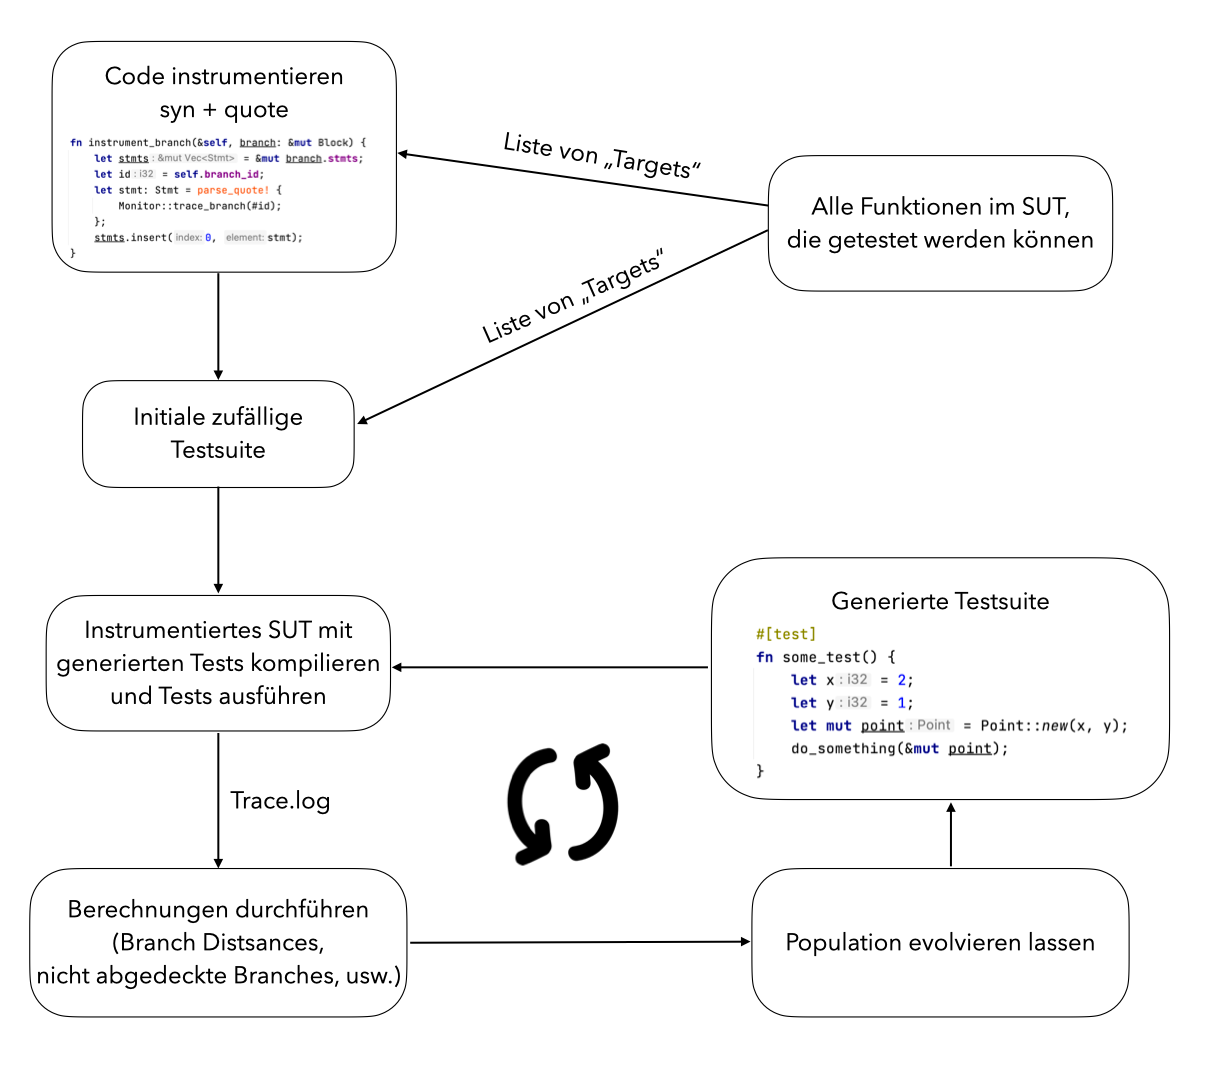
\includegraphics[width=\textwidth]{testify-overview}
\label{fig:testify-overview}
\end{figure}
\subsection{Testability Transformations}
\subsection{Instrumentation}
Tests that are generated by a search-based technique need to be executed at least once to provide some feedback on their fitness in regard to the \ac{SUT}. At this point, the coverage data and branch distances can be collected. In order to do so, the \ac{SUT} has to be instrumented with additional code, which traces the executed paths. Many other state of the art tools that generate coverage for Java instrument the bytecode of the compiled \ac{SUT} and use Reflection to run the generated tests. However, Rust compiles to machine code. Although there exist tools that allow static analysis and binary transformation, e.g., reg.ng~\cite{DiFederico2018}, the instrumentation will be done on the source code level. \textbf{syn} and \textbf{quote} are two mature libraries that allow parsing Rust code into a syntax tree and converting the tree back to regular code, respectively. 

During the instrumentation, additional tracing statements will be inserted into a \ac{SUT} to report visited branches. The original source files will be backed up and temporarily replaced by the instrumented ones. Additionally, while traversing the syntax tree, all testable data structures, as well as their constructors, fields, and methods, are captured. At the end of this process, it will be known which methods can be tested, what parameters they have, which generators can be used to instantiate those parameters, and how the parameters are used, i.e., borrowed or consumed. 

\begin{lstlisting}[language=Java, caption=Division by zero transformation, label=lst:example-testability-transformation]
fn div(a: i32, b: i32) -> f64 {
    if b == 0 {
        panic!("Dividing by zero")
    } else {
        a as f64 / b as f64
    }
}
\end{lstlisting}

Similar to Java, trait implementations in Rust must follow some standard contracts. For instance, when implementing both \lstinline{Hash} and \lstinline{Eq}, it is required that the following property holds: 
\[
k1 == k2 \longrightarrow hash(k1) == hash(k2)
\] 
i.e., if two keys are equal, their hashes must also be equal. Some of the traits in the standard library can be derived automatically, which should generate implementations that comply with an appropriate contract. However, a manual implementation might still be desirable in case some members of a struct do not implement the trait to derive, or a custom version is required. A contract violation might be considered a bug and shall be checked during the execution of generated tests, as is done in Randoop~\cite{Pacheco_2007} and EvoSuite~\cite{Fraser2013}. 

\subsection{Test Execution}
With Cargo, Rust provides a build system and a testing framework out-of-the-box. In Java, which is a managed language~\cite{Gough2005}, generated tests can be executed directly using Reflection and bytecode instrumentation, and coverage information can be collected in the same runtime process. This cannot be done that conveniently in Rust, and tests must first be compiled. Then the Cargo test framework is called on the module under test to run the tests. To speed up the process, a whole population of tests is compiled and run concurrently. To keep the exact coverage of each individual test, each test sets a \lstinline{thread_local} test ID at the beginning of its execution, which the instrumented \ac{SUT} uses during execution to trace the coverage. 

As shown in Figure~\ref{fig:test-execution}, the instrumented \ac{SUT} reports important events during its execution to the message queue of the monitor thread (MT). These are, for example, the execution of a root branch (method or function) or a decision branch. For the latter, the branch distance, which is calculated on the fly, is passed along with other data. The MT is initialized before the threads are started and can either write collected coverage data to a file or send it directly to the main process via TCP.

\begin{figure}[h]
\caption{An example concurrent execution of multiple tests with a monitor}
\centering
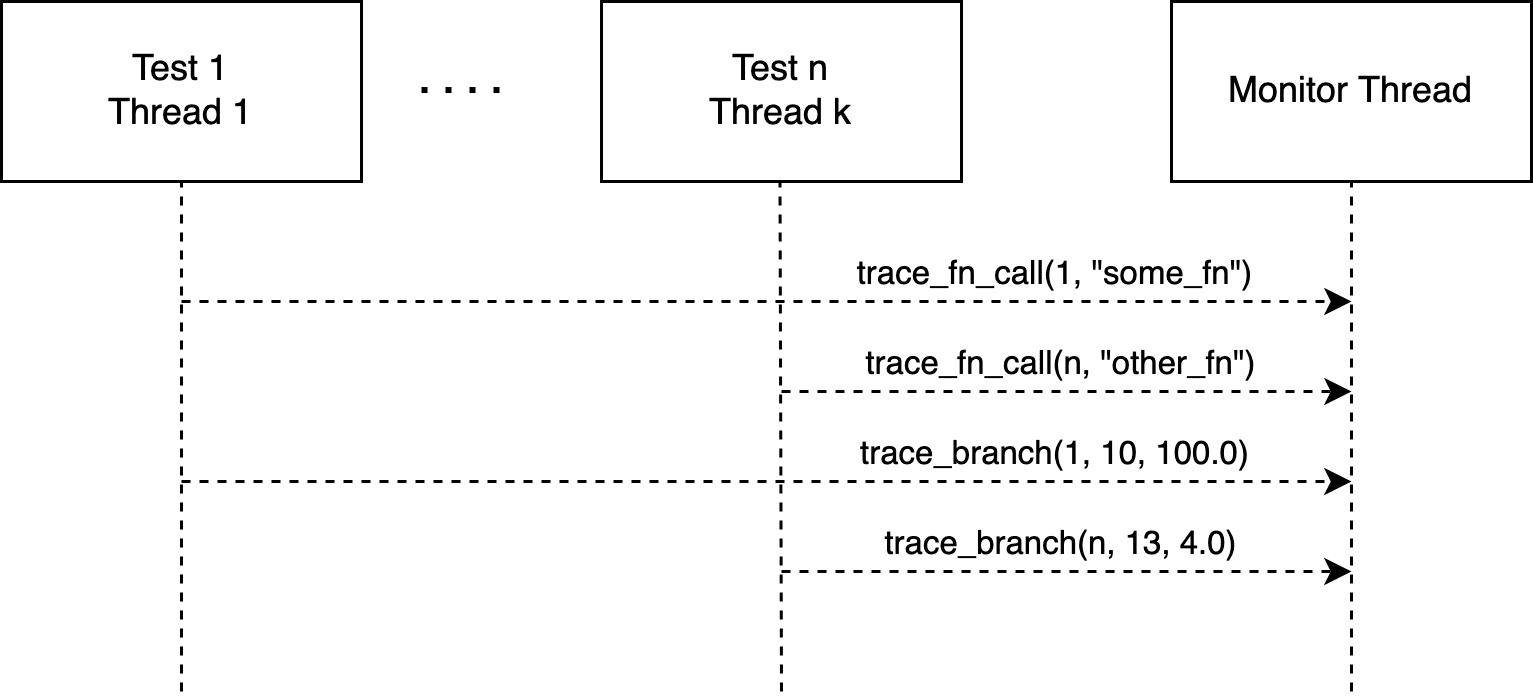
\includegraphics[width=\textwidth]{test-execution}
\label{fig:test-execution}
\end{figure}

Real and complex software often interacts with its environment, for example by making I/O calls to the file system or establishing TCP connections. Lack of handling of the execution environment the \ac{SUT} lives within is still one of the open problems in \ac{SBST}~\cite{McMinn2011}. To avoid unwanted side effects, EvoSuite~\cite{Fraser2013a} relies on strict security measures of the Java Security Manager and prohibits most interactions of \ac{SUT} with its environments. These could lead to uncontrolled behavior if executed repeatedly, such as generating countless random files or even wiping the entire disk. Only few essential operations are allowed, such as I/O for the classloader, loading libraries, or reflection. As a preprocessing step, EvoSuite extracts only those methods that return the same result when run repeatedly with the same inputs, i.e., methods that are deterministic~\cite{Fraser2012}.

KLEE~\cite{cadar2008klee} takes a different approach and redirects concrete calls, such as \lstinline{open()} and \lstinline{read()}, to \textit{models} that understand the semantics of the desired action well enough to generate the required constraints. These models are written in normal C code which the use can readily customize, extend, or even replace with their own custom implementation. Function calls are replaced in a pre-processing step in \ac{SUT} by mocks that mimic the original behavior. When the \ac{SUT} reads values from the environment, such as from a file, a legal, randomly generated value of the same type is returned as the original function would have done. When the \ac{SUT} writes to the environment, the values are stored in memory during the execution of the corresponding test such that the effect of these alterations are reflected in potential subsequent reads. 


\subsection{Test Suite Optimization}
Figure~\cref{fig:testify-overview} illustrates the main steps in the Testify Tool: It starts by instrumenting the \ac{SUT} and inserting necessary statements to trace a programm execution. Then, a random test suite is generated based on the \ac{SUT} and evolved using evolutionary search towards a specified fitness goal. At the end, the test suite with the highest coverage is returned. 

\subsubsection{Problem representation}
According to McMinn~\cite{McMinn_2004}, an encoding of the solution should be modeled in a way that similar solutions are also neighbors in the represented search space. This makes it easy to continue the search from one to a similar solution by applying simple modifications of the representation. In single-objective genetic algorithms for test generation, a chromosome in a population typically represents an entire test suite~\cite{Fraser_2011, Campos2017}. However, \acp{MOA} define a chromosome to be a single test case~\cite{Panichella2018}. Chromosome representation has a direct impact on how, for instance, the crossover operator works. Recombining two test suites is trivial by recombining only the sequences of their test cases at specific cut points since individual test cases are independent of each other~\cite{Fraser_2013}. Recombining test cases is more complicated because it means recombining their sequences of statements, which are, however, very much interdependent. For example, a statement could instantiate an object by invoking an appropriate constructor, followed by a later method invocation on that object. In the following, a chromosome is a test case, which is a sequence of statements or program calls that execute parts of the \ac{SUT} to reach and cover a certain objective. Since programs in Rust are not just procedures but have a certain class-like structure, this must also be taken into account. In a simple procedural program, tests would only need to call procedures with certain input data to achieve high coverage. However, instances of classes and (in Rust) class-like structs can have states that can be changed either directly or via method calls. The control flow graph of a method may depend on the internal state of an object. This means that a certain statement call sequence may be important to achieve high code coverage. For the generation of unit tests with a genetic algorithm, this work implements already known ideas for the representations of genetic solutions~\cite{Fraser2012,Tonella2004,Arcuri2008}. Similar to Frasers and Arcuris~\cite{Fraser_2011} definition, each statement~$s_i$ in a test case is a value~$v(s_i)$, which has a type~$\tau(v(s_i)) \in \mathcal{T}$, where~$\mathcal{T}$ is the finite set of types. There can be five different types of statements: 

\begin{itemize} 
    \item \textbf{Primitive statements} represent numeric variables, e.g., \lstinline{let v = 42}. Value and type of the statement are de- fined by the primitive variable.
    \item \textbf{Constructor statements} generate new instances of a given struct, z. B. \lstinline{let b = Book::new()}. Value and type of the statement are defined by the object constructed in the call. A constructor can have parameters whose values are assigned out of the set ~$\{v(s_k)~|~0 \leq k < i\}$. However, constructors are not part of the Rust language. Using a static method called \lstinline{new}, which returns an instance of the appropriate struct, is not mandatory but a convention. Thus, if a struct does not provide the new method, it still can be instantiated the C-like way, i.e., \lstinline|let b = Book { name: "A" }|. 
    \item \textbf{Field statements} access member variables of objects, e.g., \lstinline{let b = a.x}. Value and type of a field statement are defined by the member variable. The source of the member variable, i.e.,~\lstinline{a}, must be part of the set~$\{v(s_k)~|~0 \leq k < i\}$. Since unit tests are usually contained in the same module as the~\ac{CUT}, tests can also legally access private fields and methods. 
    \item \textbf{Method statements} invoke associative methods on objects or static methods, e.g., \lstinline{let b = a.len()}. The owner of the method (if non-static) and all of the parameters must be values in~${\{v(s_k)~|~0 \leq k < i\}}$. Value and type of a method statement are defined by its return value.
    \item \textbf{Function statements} invoke free-standing functions, e.g., \lstinline{let a = foo()}. The parameters of the function must be values in~$\{v(s_k)~|~0 \leq k < i\}$. Value and type of a function statement are defined by its return value.
\end{itemize}

The collection of available structs, their constructors, methods, fields, and free-standing functions are so-called test cluster~\cite{Fraser_2011}. The size of a test suite as well as individual tests is dynamic and can change (almost) arbitrarily. Since there will be no test oracles available for most of the generated tests, the size of the test suite, as well as the individual tests, should have an upper limit, so that test oracles can be inserted later manually. 

Each statement that does not have the default return value~\lstinline{()} defines a new variable. However, a generated test cannot be composed arbitrarily of the above building blocks. Each test is subject to the same constraints as regular Rust programs, which are checked by the compiler~\cite{Tonella2004}. Constructors, methods, functions, and fields in a test are not limited to just the parts of the module under the test since complex sequences of calls might be necessary to define some arguments~\cite{Fraser2012}. 

Rust's affine type system makes usage of already defined objects more complicated since the information in which statements a particular instance was used in which way (borrowed or consumed) must also be tracked. That is, an already defined object may be used in any way by a newly inserted statement~$s'$ only if it is marked as free to use and is not used by any other statement~$s$ that comes after~$s'$. Otherwise,~$s'$ may use the object in a way that does not collide with~$s$. More precisely, the rules are defined as follows: let~$t$ be a test case and $pos(s)$ a function that returns the position of a statement~$s$ in the sequence of statements in~$t$. Let~$o$ be an object of a data type~$c$ defined by statement~$gen$. A new statement~$s'$ is inserted, which uses~$o$. Then the following must hold:
\begin{itemize}
    \item $gen \in t \wedge pos(gen) < pos(s')$.
    \item If~$o$ is not used by any statement~$s \in t$,~$o$ may be consumed or borrowed by~$s'$. 
    \item If~$o$ is borrowed by a statement~$s \in t$,~$o$ may also be borrowed by~$s'$ at position~$p_{borrow}$ with ~$pos(gen) < p_{borrow}$ or consumed at position~$p_{consume}$ with~$pos(s) < p_{consume} < \left|t\right|$. 
    \item If~$o$ is consumed by a statement~$s \in t$,~$o$ may be borrowed by~$s'$ at position~$p_{borrow}$ with~$pos(gen) < p_{borrow} < pos(s)$. 
\end{itemize}

Initialization and usage of objects shall be tracked in a \ac{DDG} per test case, e.g., as in Listing~\ref{lst:example-test}. The nodes in the graph are statements. When a statement~$a$ depends on some other statement~$b$, it means that~$a$ actually depends on a variable whose value has been defined by~$b$. 

\begin{minipage}{0.45\textwidth}
\begin{lstlisting}[language=Java, caption=An example test, label=lst:example-test]
let a = A::new();   // Id: stmt_a
let b = B::new(&a); // Id: stmt_b
let c = C::new();   // Id: stmt_c

a.foo(&b);          // Id: stmt_d
b.bar(c);           // Id: stmt_e
\end{lstlisting}
\end{minipage}%
\hfill
\begin{minipage}{0.45\textwidth}
\begin{figure}[H]
  \caption{The DDG of the example test}

  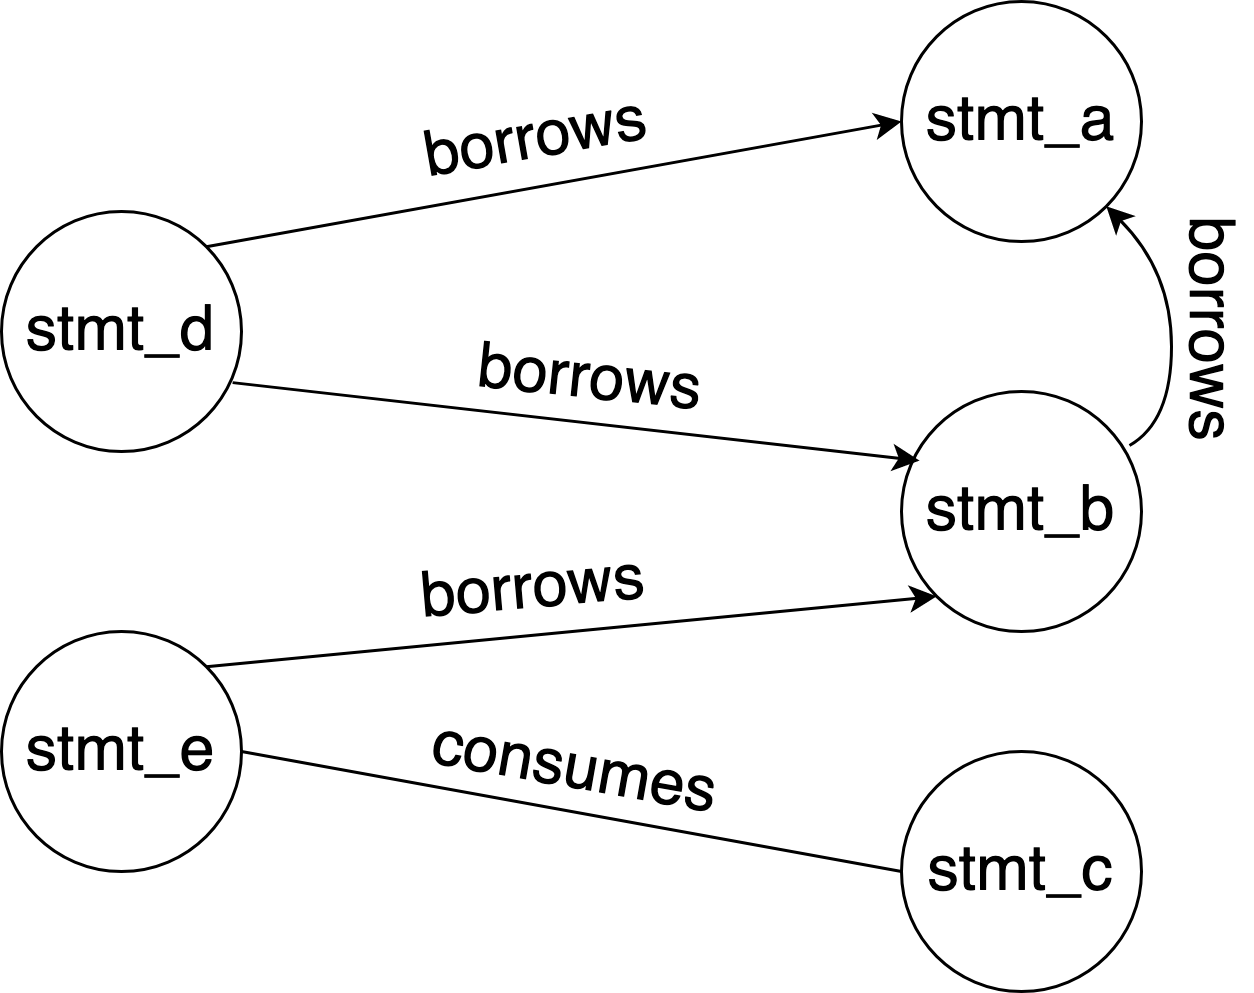
\includegraphics[width=\linewidth]{ddg-expose}
\end{figure}
\end{minipage}%

Fraser und Zeller~\cite{Fraser2012} beschreiben in ihrer Arbeit zum Mutations-basiertem Generieren von Tests für Java Klassen ein abstraktes Konstrukt, welches die Modellierung und Aufbau eines Unit Tests leicht veranschaulicht. Sei~$parameters(M)$ eine Funktion, die eine Liste von Datentypen der Parameter einer Methode oder Funktion~$M$ zurückgibt, einschließlich des Aufrufers im Falle einer nicht-statischen Methode. Des Weiteren, sei~$classes(t)$ eine Funktion, die den Set von Datentypen zurückgibt, dessen Objekte in einem Test~$t$ bereits instanziert wurden. Eine Funktion oder eine Methode ist ein Generator eines Datentyps~$C$ wenn sie einen Rückgabewert vom Typ~$C$ haben. Außerdem ist jeder Konstruktor eines Structs vom Typ~$C$ ebenfalls ein Generator von~$C$. Sei~$generators(M,C)$ eine Funktion, die den Set von Generatoren für den Datentyp~$C$ aus dem Set von Methoden und Funktionen~$M$ zurückgibt. 

\begin{algorithm}[t]
\caption{$GenTest(M, l)$}\label{alg:random-generation-of-a-test}
\begin{algorithmic}
\Input
  \Desc{$M$}{Set of all method, constructors and functions}
  \Desc{$l$}{Desired length of a test case}
\EndInput
\Output
  \Desc{$t$}{Randomly generated test}
\EndOutput    
\State{$t \gets \langle\rangle$}
\State{$s \gets$ randomly select an element from M}


\For{$p \in parameters(s)$}
  \State{$t \gets GenObject(p, \{\}, M, t)$}
\EndFor
\State{$t \gets t.s$}

\While{$\left|t\right| < l$}
  \State{$c \gets$ randomly select datatype in $classes(t)$}
  \State{$M' \gets \{m | m \in M \wedge c \in parameters(m)\}$}
  \State{$s \gets$ randomly select method or function from $M'$}
  \For{$p \in parameters(s)$}
    \If{$\neg(p \in classes(t))$}
      \State{$t \gets GenObject(p, \{\}, M, t)$}
    \EndIf
  \EndFor
  \State{$s \gets$ set parameters of $s$ to values from $t$}
  \State{$t \gets t.s$}
\EndWhile
\State \Return $t$
\end{algorithmic}
\end{algorithm}


Die initiale Population wird zufällig generiert, wie im Algorithmus~\labelcref{alg:random-generation-of-a-test} dargestellt. Bevor die Tests generiert werden, werden alle verfügbaren Methoden, Konstruktoren und Funktionen, sowie Attribute von Structs statisch extrahiert. Bei einem zufällig generierten Test wird daraus ein zufälliger Aufruf eingefügt. Die evtl. notwendigen Argumente (inklusive des Aufrufers) werden dabei ebenfalls generiert. Dafür werden entsprechende Aufrufe, die Rückgabewerte von passenden Datentypen haben, rekursiv eingefügt (Algorithmus~\labelcref{alg:random-generation-of-args}), wenn im Test Case nicht bereits Instanzen eines solchen Datentyps definiert sind. Während der Suche werden die Datentypen, die zu instanziieren bereits versucht wird, gemerkt, um unendliche Rekursionen zu vermeiden. Laut den Algorithmen~\labelcref{alg:random-generation-of-a-test} und~\labelcref{alg:random-generation-of-args} werden neue Objekte nur dann generiert, wenn sie nicht im Test bereits existieren. Fraser und Zeller~\cite{Fraser2012} schlagen jedoch vor, bestehende Objekte nur mit einer gewissen Wahrscheinlichkeit wiederzuverwenden, um Diversität in generierten Test Cases zu erhöhen. In ihren Experimenten haben sie festgestellt, dass eine Wahrscheinlichkeit von 90\% Prozent am effektivsten ist. Rusts affines Typsystem macht eine Wiederverwendung von bereits definierten Objekten komplizierter, da die Information, in welchen Aufrufen eine bestimmte Instanz auf welche Weise verwendet wurde (ausgeliehen oder konsumiert) ebenfalls mitgeführt werden muss. Das heißt, dass ein bereits definiertes Objekt nur dann von einem neu eingefügten Statement~$s$ verwendet werden darf, wenn es als frei verwendbar markiert ist und von keinem anderen Statement verwendet wird, das nach~$s$ kommt. Genauer werden die Regeln folgenderweise definiert: Sei~$t$ ein Test Case und $pos(s)$ eine Funktion, die die Position eines Statements~$s$ in der Sequenz von~$t$ zurückgibt. Sei~$o$ ein Objekt von einem Datentyp~$c$, das von einem Statement~$gen$ definiert wird. Ein neues Statement~$s'$ wird eingefügt, welches~$o$ verwendet. Es gilt für die Positionen:~$pos(gen) < pos(s')$. Außerdem gilt:
\begin{itemize}
    \item Wenn~$o$ von keinem Statement~$s \in t$ verwendet wird, darf~$o$ von~$s'$ konsumiert und ausgeliehen werden. 
    \item Wenn~$o$ von einem Statement~$s \in t$ ausgeliehen wird, darf~$o$ von~$s'$ an der Position~$p_{borrow}$ mit ~$pos(gen) < p_{borrow}$ ebenfalls ausgeliehen oder an der Position~$p_{consume}$ mit~$pos(s) < p_{consume} < \left|t\right|$ konsumiert werden. 
    \item Wenn~$o$ von einem Statement~$s \in t$ konsumiert wird, darf~$o$ von~$s'$ an der Position~$p_{borrow}$ mit~$pos(gen) < p_{borrow} < pos(s)$ ausgeliehen werden. 
\end{itemize}
Das Ganze wird mit Hilfe eines Data Dependence Graphen realisiert, in dem jedes Statement bzw. ein definiertes Objekt die Rolle eines Knoten hat und Beziehungen wie z. B. \textit{Consumes} oder \textit{Borrows} zwischen Statements und ihren Argumenten notiert werden können. 


Fraser und Zeller schlagen ebenfalls vor, wenn sich eine zufällige Generierung als schwierig erweist, kann Algorithmus~\labelcref{alg:random-generation-of-args} in eine umfassende Suche mit Backtracking umgewandelt werden. Auch wenn der Suchraum groß ist, sei das gar kein so großes Problem, da Teilsequenzen zur Generierung von Instanzen wiederverwendet werden können. Die Test Cases werden so lange auf diese Weise produziert, bis die gewünschte Größe der Population erreicht ist. 



\begin{algorithm}[t]
\caption{$GenObject(c, G, M, t)$}\label{alg:random-generation-of-args}
\begin{algorithmic}
\Input
  \Desc{$c$}{Datatype of desired object}
  \Desc{$G$}{Set of datatypes already attempting to generate}
  \Desc{$M$}{Set of all method, constructors and functions}
  \Desc{$t$}{Test case}
\EndInput
\Output
  \Desc{$t$}{Test case extended with an instance of $c$}
\EndOutput    
\State{$M' \gets generators(M, c)$}
\State{$s \gets$ randomly select an element from M'}

\For{$c \in parameters(s)$}
  \If{$\neg(c \in classes(t))$}
    \State{$t \gets GenObject(c, G, M, t)$}
  \EndIf
\EndFor
\State{$s \gets$ set parameters of $s$ to values from $t$}
\State{$t \gets t.s$}
\State \Return $t$
\end{algorithmic}
\end{algorithm}

\subsubsection{Bloat Control}
Hier wird beschrieben, wie man verhindern kann, dass die Größe der Test Suite und einzelner Tests ausartet. Fraser und Arcuri~\cite{Fraser_2011} haben ein paar Gedanken dazu. 

\subsubsection{Search Operators}
The evolution of a population is performed by repeated selection of test cases and applying crossover and mutation operators according to a certain probability~\cite{Fraser2012}.

There are different selection methods, e.g., fitness-proportional selection, linear ranking, or tournament selection~\cite{McMinn_2004}. The key is to guide the search towards solutions with better fitness values. Once the set of parents has been selected, recombination (or crossover) can take place to form the next generation. Crossover is applied to individuals with a certain probability. The most basic recombination is a single point crossover, where a random position in each of the two selected test cases is selected, and new test cases (offspring) are generated by swapping the subsequences of statements~\cite{Fraser2012}. At this point, the dependencies of the statements will be considered, and possibly missing arguments will be generated in the offspring test cases. In addition, the \acp{DDG} of those test cases must also be adjusted.

After selection and crossover have been applied, the offspring can mutate. There are different ways of mutation, e.g., delete, insert, or modify a statement~\cite{Fraser2012}. Modifying a statement includes changing the callee of a method, parameters, or replacing the method itself with another one. The \ac{DDG} of each test case determines what mutation is possible, e.g., replacing a method call to \lstinline{fn foo(&self)} by \lstinline{fn bar(self)} is not allowed if the callee of the method is also used by some other statement later in the sequence because the \lstinline{bar} method consumes the callee. 

\subsubsection{Mutation}
Chromosome werden hier in ihrer ''natürlichen'' Weise repräsentiert, also nicht in der Binärform. Das heißt für einen Test Case, dass er aus einer Sequenz von Statements besteht. Diese können auf verschiede Weisen mutiert werden: 

\textbf{Insert a method or function invocation}: Ein neuer Methodenaufruf wird dem Test Case hinzugefügt. Die von der Methode benötigten Argumente werden ebenfalls, wenn nötig initialisiert, und hinzugefügt. Eine Variable wird zufällig ausgewählt, deren Methode aufgerufen werden soll, oder ein neues Objekt wird zuvor erstellt, mit einem Datentypen, welcher im jeweiligen Test bereits verwendet wurde~\cite{Fraser2012}. Der Aufruf wird zufällig zwischen dem Initialisieren des Objects und dem Aufruf der \ac{MUT} eingefügt (falls man überhaupt von einem festgesetzten MUT, also bottom-up, ausgeht). Es können auch mehrere Methodenaufrufe wiederholt eingesetzt werden, wobei dies mit der Wahrscheinlichkeit~$p(n) = 0.5^n$ passiert, wo $n$ die Anzahl von bisher eingefügten Aufrufen ist. Das heißt, dass nach jedem Einsetzten eine zufällige Entscheidung getroffen wird, ob die Mutation wiederholt werden soll~\cite{Tonella2004}.
\begin{lstlisting}[language=Java, caption=, label=lst:mutation-invocation-insertion]
let a = A::new();
a.m(10, 5);

// wird zu 
let a = A::new();
let b = B::new();
a.f(b);
a.m(10, 5);
\end{lstlisting}

\textbf{Delete a method or function invocation}: Einige Methodenaufrufe können zufällig aus einem Test Case gelöscht werden. Werte, die dadurch im Test Case nicht mehr verwendet werden, werden ebenso gelöscht. Falls das gelöschte Statement~$s$ einen Rückgabewert hatte, welcher von einem anderen Statement~$s'$ verwendet wird, muss~$s'$ entweder ebenfalls gelöscht werden oder das entsprechende Argument durch ein anderes, im Test bereits definiertes Objekt des gleichen Datentyps ersetzt werden~\cite{Fraser2012}.
\begin{lstlisting}[language=Java, caption=, label=lst:mutation-invocation-removal]
let a = A::new();
let b = B::new();
a.f(b);
a.m(10, 5);

// wird zu 
let a = A::new();
a.m(10, 5);
\end{lstlisting}
Der Aufruf von \lstinline{a.f(b)} wurde zufällig zum Löschen ausgewählt. Da es die einzige Stelle war, an der \lstinline{b} verwendet wurde, wurde es ebenfalls gelöscht. Ähnlich wie das Einsetzen von Methodenaufrufen, kann dieser Operator mit der Wahrscheinlichkeit~$p(n) = 0.5^n$ wiederholt angewendet werden, wobei $n$ die Anzahl von gelöschten Statements ist. 

\textbf{Modify an existing statement}: Eine der folgenden Veränderungen wird angewendet~\cite{Fraser2012}:
\begin{itemize}
  \item \textit{Change callee:} For a method call or field reference, change the source object.
  \item \textit{Change parameters:} Change one parameter of a method, constructor or function call to a different value or create a new value.
  \item \textit{Change method/constructor/function:} Replace a call with a different one with an identical return type.
  \item \textit{Change field:} Replace a primitive value with a different primitive value of the same type.
\end{itemize}
\begin{lstlisting}[language=Java, caption=, label=lst:mutation-input-value]
let a = A::new();
a.m(10, 5);

// wird zu 
let a = A::new();
a.m(20, 5);
\end{lstlisting}

\subsubsection{Crossover}
Die einfachste Art von Crossover ist der One-Point-Crossover, so wie er in~\cref{sec:background-crossover} beschrieben ist. Die Chromosome werden hier jedoch in der natürlichen Art repräsentiert, als Sequenz von Statements, was dazu führt, dass beim Aufteilen und Durchtauschen von Köpfen eines Paars von Chromosomen auf die Abhängigkeiten der Statements geachtet werden muss. Tonella~\cite{Tonella2004} schlägt zwei Alternativen vor:
\begin{itemize}
    \item Fehlende Abhängigkeiten von Statements können wie beim Mutationsoperator durch das Generieren ergänzt werden. \todo{Beispiel} Sollten bestimmte Definitionen dadurch überflüssig werden, dass ihre spätere Benutzung durch Rekombination in ein anderes Choromosom geschoben wurde, können diese gelöscht werden. 
    \item Abhängigkeiten von einem durch Rekombination verschobenen Teil eines Chromosoms werden unabhängig vom Crossover-Point ebenfalls in ein anderes Chromosom geschoben, sofern diese im ursprünglichen Chromosom nicht mehr benötigt werden. \todo{Beispiel}
\end{itemize}

\subsubsection{Dependencies}
Hat man beispielsweise ein Rust Programm wie in Listing~\ref{lst:example-rust-program}, welches raus einem Struct für Rechtecke und einem Struct, welcher Operationen auf dem Rechteck durchführt (was nicht ganz der guten Sitten des Software Engineering entspricht, daher sollte ein besseres Beispiel hergenommen werden). 

\begin{lstlisting}[language=Java, caption=Ein Beispiel für ein Rust Program, label=lst:example-rust-program]
struct Rectangle {
    width: u64,
    height: u64,
}

impl Rectangle {
    pub fn new(width: u64, height: u64) -> Self {
        Rectangle { width, height }
    }
    pub fn width(&self) -> u64 {
        self.width
    }
}

struct Calculator {}

impl Calculator {
    pub fn new() -> Self {
        Calculator {}
    }
    pub fn area_by_value(&self, r: Rectangle) -> f64 {
        r.height as f64 * r.width as f64
    }
}
\end{lstlisting}
Ein Beispiel Testcase für das Program kann wie im Listing~\ref{lst:example-testcase} aussehen. Dabei wird ein Rechteck mit einer bestimmten Länge und Breite erstellt und vom Calculator konsumiert, um die Fläche des Rechtecks zu bestimmen. Das affine Typsystem von Rust erlaubt es nicht,\todo{Verschiedene Typsysteme in einer kleinen Übersicht erklären?} dass die Variable~\lstinline{calculator_0} noch mal verwendet wird. Es kann also nach dem Statement in der Zeile 4 weder auf die Attribute von dem Recheck zugegriffen werden, noch kann das Rechteck als Argument für weitere Aufrufe dienen. 
\begin{lstlisting}[language=Java, caption=Ein Beispiel Testcase, generiert für das Program im Listing~\ref{lst:example-rust-program}, label=lst:example-testcase]
let mut rectangle_0 = Rectangle::new(205u8, 166u8);
let u64_0 = rectangle_3.width();
let mut calculator_0 = Calculator::new();
let f64_4 = areacalculator_0.area_by_value(rectangle_0);
\end{lstlisting}
Die im Testcase aus dem Listing~\ref{lst:example-testcase} können mit einer Art von Data-Dependence-Graph wie in Figure~\ref{fig:ddg-example}.

\begin{figure}[h]
\caption{Data-Dependence-Graph für den Testcase aus dem Listing~\ref{lst:example-testcase}}
\centering
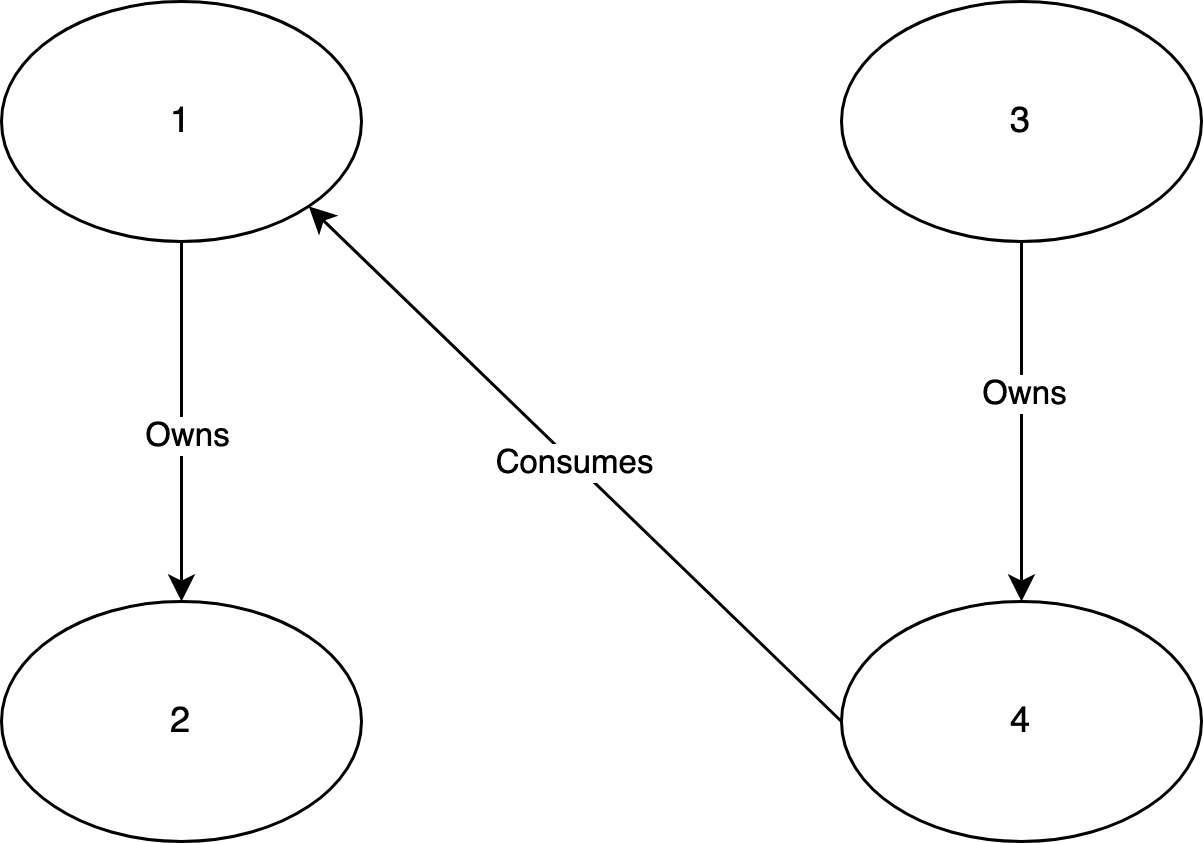
\includegraphics[width=\textwidth]{DDG}
\label{fig:ddg-example}
\end{figure}

\subsubsection{Fitness Function}
Um die Selektion von Parents für die nachkommende Generationen besser guiden zu können, werden alle Individuen in einer Population nach ihrer Fitness ausgewertet. Eine gute Fitnessfunktion ist sehr wichtig bei der Suche nach Lösungen. Lösungen, die in einer bestimmten Weise \"besser\" als andere sind, sollen mit besseren Fitnesswerten belohnt werden. Was auch immer eine bessere Fitness ist, eine höhere oder niedrigere Fitness hängt davon ab, ob die Suchstrategie versucht, die Fitnessfunktion zu maximieren oder zu minimieren~\cite{McMinn_2004}. Dieser Ansatz wird sich voraussichtlich auf Branch Coverage konzentieren. EvoSuite instrumentiert in der originalen Implementierung Java SUT auf Bytecode-Level und im Bytecode werden alle Loops usw. in die einfachen if-Verzweigungen überführt. Das Ziel ist es, die optimale Lösung zu finden, d. h. eine Test Suite, die möglichst hohe Branch-Coverage hat. Gleichzeitig soll es aber keine andere Testsuite geben, die bei gleicher Branch-Coverage kleiner ist bzw. kleinere Tests enthält. Einige Branches, sogenannte infeasible Branches, können evtl. gar nicht abgedeckt werden, entweder aufgrund der limitierten Repräsentation der Lösung oder weil es keine passenden Inputs existieren. Somit werden solche Tests bevorzugt bei der Evolvierung bevorzugt, die eine höhere Fitness bzgl. der Branch-Coverage haben. Bei zwei Tests mit der gleichen Coverage wird der kürzere bevorzugt. 

Um die Suche voranzutreiben, können verschiedene Heuristiken verwendet werden. \todo{Welche gibt es überhaupt?} Eine der weitverbreitesten ist Branch Distance. McMinn~\cite{McMinn_2004} beschreibt eine Sammlung von Regeln, die rekursiv angewendet werden können, um Distanz bei allen möglichen Prädikaten zu berechnen. Wenn die Ausführung des \ac{SUT} bei gegebenen Inputdaten in einem bestimmten Branch landet, so kann eine lokale Suche angewendet werden. Es wird mit Hilfe einer lokalen Fitnessfunktion abgeleitet, wie nah das Prädikat zum Auswerten zu \lstinline{true} ist. Zum Beispiel, bei einem Prädikat~\lstinline{x >= 10} und~\lstinline{x = 5} (während der Ausführung) wird der \lstinline{false} Branch getroffen. Die Distanz zum \lstinline{true} Branch beträge somit~$10 - 5 + k$ mit~$k \geq 1$. Dabei wird jedes Prädikat im \ac{SUT} instrumentiert, um die Distanzen zu anderen Branches während der Ausführung des \ac{SUT} zu tracen. Die Branch-Distanz muss noch normalisiert werden (je nach Werten kann es schnell zu Extremen kommen). Arcuri~\cite{Arcuri_2011} beschreibt in seiner Arbeit, welchen Einfluss die Normalisierung der Branch-Distanz auf die Effektivität einer such-basierten Testgenerierung hat. 

\subsection{Test Oracles and Testability Transformations}
Traditionally, \ac{SBST} is applied to generate test suites that maximize some coverage criteria, e.g., in this case, branch coverage. However, search-based techniques usually do not make any use of automated oracles~\cite{Fraser2013}. A lack of formal specification of the behavior of a program results in generated tests that must be supplemented with oracles manually. A technique called \textit{testability transformation} tries to overcome this obstacle. A testability transformation is a source-to-source program transformation that seeks to improve the performance of some chosen test data generation technique~\cite{Harman2004}, e.g., reach difficult branches. Beyond that, a \ac{SUT} can be transformed in a way such that artificial branches are inserted into the code to guide the search into triggering some exceptional behavior and crash the program. For instance, EvoSuite~\cite{Fraser2013} employs multiple testability transformations such as array access transformation, division by zero transformation, or numerical overflow transformation. Those transformations do not increase code coverage in general but contribute to discovering potential unforeseen behavior and generating inputs that trigger it. Similar transformations can also be applied for Rust and shall be part of the approach. Even though EvoSuite transforms the bytecode of a \ac{SUT} to apply testability trasnformations, this can also be done on the source code level in Rust as done in Listing~\ref{lst:example-testability-transformation}.

\subsection{Test Minimization}
%Da sich diese Arbeit vor allem auf das Generieren vor Tests beschränkt, die möglichst hohe Coverage erreichen, jedoch generell keine Testorakel automatisch zur Verfügung stellt, sollen die Tests möglich kurz gehalten werden und das wesentliche tun, um einen bestimmten Branch zu erreichen. Das erhöht ihre Lesbarkeit und Verstänlichkeit. Fraser und Arcuri~\cite{Fraser2013a} schlagen als Verbesserung für ihr EvoSuite Tool folgendes Verfahren vor: Für jeden Coverage Goal wird ein Test aus der generierten Test Suite ausgewählt, der diesen Goal abdeckt. Dieser Test wird wrt to the coverage goal minimiert, so dass Statements, die nicht zur Ausführung des Goals beitragen, gelöscht werden. Wenn ein Goal bereits von einem minimierten Test abgedeckt ist, so wird kein weiterer Test für diesen Goal der finalen Test Suite hinzugefügt. Auf diese Weise werden Tests lesbarer für einen Menschen und können somit leichter manuell um Testorakel ergänzt werden. 

Since this work is mainly limited to generating tests that achieve the highest possible coverage but do not provide test oracles automatically in general, the tests should be kept as short as possible and do the essential to achieve a certain branch. This increases their readability and comprehensibility. Fraser and Arcuri~\cite{Fraser2013a} propose the following procedure as an improvement for their EvoSuite tool: for each coverage goal, a test is selected from the generated test suite that covers that goal. That test is minimized with respect to the coverage goal so that statements that do not contribute to the execution of the target are removed from the test. If a target is already covered by a minimized test, no further test for this objective will be added to the final test suite. This way, tests become more readable to a human and can thus be more easily supplemented manually with test oracles. 

\subsection{Usability}
EvoSuite scheint sehr auf Usability ausgerichtet zu sein, zum Beispiel gibt es ein Eclipse Plugin, welches man per Click zum Generieren von Tests für das offene Projekt benutzen kann. Außerdem, da SBST mit Iterationen arbeitet, kann man die Ausführung jederzeit beenden und die bisher besten Ergebnisse zurück geben~\cite{Harman2015}. Das obere Limit für die Ausführungszeit von generierten Tests ist in diesem Kontext von Bedeutung. 
\section{Evaluation}
To determine how well a search-based approach performs with respect to code coverage and program crash detection, a set of experiments shall be conducted on a set of open-source Rust software, e.g., libraries. As there is already another tool available, KLEE, which uses \ac{DSE} and can also generate tests for Rust, it can be used in the experiments. KLEE-generated tests do not depend on the tool itself and can be executed outside of it the usual way. This opens the possibility to compute a source-based code coverage available in the Rust compiler for both tools. The experiments should answer the following questions: 

%Symbolic execution often has problems constructing nice test suites with complex types, which is why this technique is rather applied to find bugs in a \ac{SUT}, than generate tests with high coverage. Seach-based approach do the opposite, they are good at generating tests with high coverage, but are not as good at finding bugs as they do not make use of test oracles~\cite{Fraser2013}.

\begin{enumerate}[start=1, label={\bfseries RQ\arabic*:}]
    \item How many program crashes and generic contact violations can be found with \ac{SBST} in open source Rust software?
    \item Does an \ac{SBST} approach achieve a higher code coverage than a \ac{DSE}-based one?
    \item Does an \ac{SBST} approach achieve a higher code coverage than manually written tests in open-source Rust software?
\end{enumerate}
To this end, a set of real Rust programs shall be chosen for experiments. The programs for experiments must comply with the following prerequisites:
\begin{itemize}
    \item There is no concurrency involved, as it introduces non-determinism and flakiness in the tests.
    \item The programs do not make use of \textit{unsafe} Rust and do not depend on external bindings, e.g., to C or C++.
    \item The programs do not interact with the execution environment, e.g., open read or write files.
    \item The programs already contain a manually written test suite that can be used in the evaluation to compare the coverage of the generated tests. 
    \item The programs use only Rust's \textit{stable} language features.
\end{itemize}

\subsection{Setup}
\subsection{Threats to Validity}
\subsection{Code Coverage Comparison with Manually Written Tests}
\subsection{Code Coverage Comparison with KLEE}


\section{Conclusion}

\section{Future Work}

\appendix
\chapter{Acronyms}
\begin{acronym}
	\acro{SUT}{System Under Test}
	\acro{CUT}{Class Under Test}
	\acro{MUT}{Method Under Test}
	\acro{SMT}{Satisfiability Modulo Theories}
	\acro{GA}{Genetic Algorithm}
	\acro{EA}{Evolutionary Algorithm}
	\acro{MOSA}{Many-Objective Sorting Algorithm}
	\acro{DynaMOSA}{Many-Objective Sorting Algorithm with Dynamic target selection}
	\acro{WS}{Whole Suite}
	\acro{WSA}{Whole Suite with Archive}
	\acro{SBST}{Search-based Software Testing}
	\acro{SBSE}{Search-based Software Engineering}
	\acro{ATP}{Automated Theorem Prover}
	\acro{DSE}{Dynamic Symbolic Execution}
	\acro{IR}{Intermediate Representation}
	\acro{MOA}{Multi- and Many-Objective Algorithm}
	\acro{DDG}{Data Dependence Graph}
	\acro{HIR}{High-level Intermediate Representation}
	\acro{THIR}{Typed HIR}
	\acro{MIR}{Mid-level Intermediate Representation}
	\acro{AST}{Abstract Syntax Tree}
	\acro{CFG}{Control Flow Graph}
	\acro{CDG}{Control Dependence Graph}
	\acro{API}{Application Programming Interface}
	\acro{NSGA-II}{Non-dominated Sorting Genetic Algorithm II}
	\acro{TCP}{Transmission Control Protocol}
	\acro{SSA}{Static Single Assignment}
\end{acronym}


\bibliographystyle{unsrt}
\bibliography{bibliography}
%\nocite*{}
\end{document}